\chapter[Engineering Mathematics]{Engineering Mathematics}
Engineering Mathematics is one of the key subject related to all other subjects. In GATE, this subject has a good weightage of around 13-14 marks. This document contains all the concepts, formulas and key notes for all the chapters in the syllabus of GATE 2023 Mechanical Engineering.\\
The most common type of questions from each unit is given in the below mentioned figure.
\begin{figure}[h!]
    \centering
    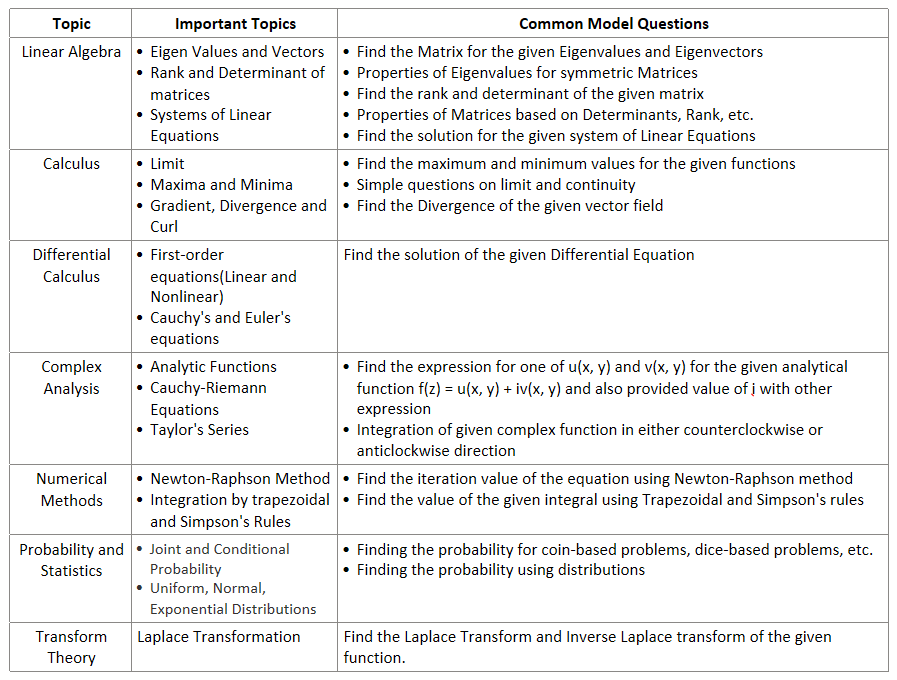
\includegraphics[width=\linewidth]{images/engineering-mathematics.png}
\end{figure}


% Section 1
\chapter*{Linear Algebra}
\section{Linear Algebra}

\subsection{Basic Matrix Operations}
Let A be a matrix of size 3x3, A = 
$\begin{bmatrix}
a_{11} & a_{12} & a_{13}\\
a_{21} & a_{22} & a_{23}\\
a_{31} & a_{32} & a_{33}
\end{bmatrix}$

\begin{itemize}
    \item Inverse of a Matrix: \(A^{-1}=\frac{1}{|A|}adj(A)\)
    \item \(adj(A) = C^T\), C = 
    $\begin{bmatrix}
        +\begin{vmatrix} a_{22} & a_{23}\\ a_{32} & a_{33} \end{vmatrix} &
        -\begin{vmatrix} a_{21} & a_{23}\\ a_{31} & a_{33} \end{vmatrix} &
        +\begin{vmatrix} a_{21} & a_{22}\\ a_{31} & a_{33} \end{vmatrix} & \\
        -\begin{vmatrix} a_{12} & a_{13}\\ a_{32} & a_{33} \end{vmatrix} &
        +\begin{vmatrix} a_{11} & a_{13}\\ a_{31} & a_{33} \end{vmatrix} &
        -\begin{vmatrix} a_{11} & a_{12}\\ a_{31} & a_{32} \end{vmatrix} & \\
        +\begin{vmatrix} a_{12} & a_{13}\\ a_{22} & a_{23} \end{vmatrix} &
        -\begin{vmatrix} a_{11} & a_{13}\\ a_{21} & a_{23} \end{vmatrix} &
        +\begin{vmatrix} a_{11} & a_{12}\\ a_{21} & a_{22} \end{vmatrix} &
    \end{bmatrix}$
    \item LU Decomposition - given matrix A is reduced to Lower L and Upper U triangular matrix 
    [A=LU]
        \begin{itemize}
            \item Crout's method (Strict last column operation)\\
            Column-wise Elementary transformation (one element at a time) can be used to obtain lower triangular matrix L. The Constants used for deducing matrix L is used to create upper triangular matrix U by replacing the specific constant (K). \\ A = LU = 
            $\begin{bmatrix} l_{11} & 0\\ l_{21} & l_{22} \end{bmatrix}$
            $\begin{bmatrix} 1 & u_{12}\\ 0 & 1 \end{bmatrix}$
            \(C_i \rightarrow C_i + KC_j\)
            \item DooLittle's method (Strict last row operation)\\
            Row-wise Elementary transformation (one element at a time) can be used to obtain upper triangular matrix U. The Constants used for deducing matrix U is used to create lower triangular matrix L by replacing the specific constant (K).\\ A = LU = 
            $\begin{bmatrix} 1 & 0\\ l_{21} & 1 \end{bmatrix}$
            $\begin{bmatrix} u_{11} & u_{12}\\ 0 & u_{22} \end{bmatrix}$ 
            \(R_i \rightarrow R_i + KR_j\)
        \end{itemize}
\end{itemize}


\subsection{Rank of a Matrix}
It is defined as the number of non-zero rows present after obtaining eucleon form of the given matrix. Rank of the matrix is evaluated using Elementary Transform method(Row or Column) or Minor method.\vspace{0.5cm}\\
\textbf{Properties}
\begin{itemize}
    \item For a null matrix '0' of any order rank(0) = 0
    \item For a non-zero matrix of order n*n; \(1 \leq rank(A) \leq n\)
    \item For a non-zero \& singular matrix \(1 \leq rank(A) < n\)
    \item For a non-zero \& non singular matrix \(A_{n*n} rank(A) = n\)
    \item For a non-zero rectangular matrix A of order m*n \(1\leq rank(A)\leq min(m,n)\)
    \item Rank of a matrix A is equal to Rank of transpose of A \(\rho(A) = \rho(A^T) \)
    \begin{table}[h!]
    \centering
    \setlength{\tabcolsep}{1em}
    \tabulinesep=1.5mm
    \begin{tabu}{c c}
    \textbf{\(\rho(A_{n*n}\))} & \textbf{\(\rho(adj(A))\)} \\
    n                          & n                         \\
    n-1                        & 1                         \\
    \textless{}n-1             & 0                         \\
    \end{tabu}
    \end{table}
\end{itemize}


\subsection{System of Linear Equation}
Consider the following system of linear equation with three variables.\\
\[a_{11}x + a_{12}y + a_{13}z = b1; a_{21}x + a_{22}y + a_{23}z = b2; a_{31}x + a_{32}y + a_{33}z = b3;\]
The system of linear equation can be represented as matrices \textbf{AX = B} as mentioned below.
\begin{center}
    $\begin{bmatrix}
    a_{11} & a_{12} & a_{13}\\
    a_{21} & a_{22} & a_{23}\\
    a_{31} & a_{32} & a_{33}
    \end{bmatrix}$
    $\begin{bmatrix} x\\ y\\ z \end{bmatrix}$ = 
    $\begin{bmatrix} b1\\ b2\\ b3 \end{bmatrix}$\\
\end{center}
In this matrix A is co-efficient matrix, X is variable co-efficient matrix and B is constant column matrix. If B = 0, then it is known as homogeneous system and If \(B \neq 0\), then the given equations form non-homogeneous system.

\subsection*{Homogeneous System [AX=0]}
\begin{itemize}
    \item Trivial Solution(Zero Solution) if \(|A| \neq 0\)
    \item Non-Trivial Solution(many Solution) if \(|A|= 0\)
    \item Number of Independent Solution = no of variables(n) - rank of matrix(p)
\end{itemize}

\subsection*{Non-homogeneous System [AX=B]}
Consider a \textbf{2x2 Matrix} with the system of linear equations.
\[a_1x+b_1y=c_1;\ a_2x+b_2y=c_2\]
The solution for these equation are given by
\begin{itemize}
    \item if \(\frac{a1}{a2}\neq \frac{b1}{b2}\) system is consistent and have a unique solution.
    \item if \(\frac{a1}{a2}=\frac{b1}{b2}=\frac{c1}{c2}\) system is consistent and have infinitely many solution.
    \item if \(\frac{a1}{a2}=\frac{b1}{b2}\neq\frac{c1}{c2}\) system is inconsistent and have no solution.
\end{itemize}
\vspace{0.2cm}Consider a \textbf{3x3 Matrix} with the system of linear equations.
\[a_{11}x + a_{12}y + a_{13}z = b1; a_{21}x + a_{22}y + a_{23}z = b2; a_{31}x + a_{32}y + a_{33}z = b3;\]
Then Matrix C is given by 
    C = [A:B]    C =
    $\begin{bmatrix}
    a_{11} & a_{12} & a_{13} & b1\\
    a_{21} & a_{22} & a_{23} & b2\\
    a_{31} & a_{32} & a_{33} & b3
    \end{bmatrix}$
    \begin{fleqn}
    \[\rho(A)=p;\ \rho(c)=r;\ \text{n - no of variables}\]
    \end{fleqn}
The solution for these equations are given by
\begin{itemize}
    \item if \(r=p=N\), then the system is consistent and has unique solution.
    \item if \(r=p<N\), then the system is consistent and has infinetly many solution.
    \item if \(r\neq p\), then the system is inconsistent and has no solution.
\end{itemize}


\subsection{Eigen Values \& Eigen Vectors}
\begin{figure}[h!]
    \centering
    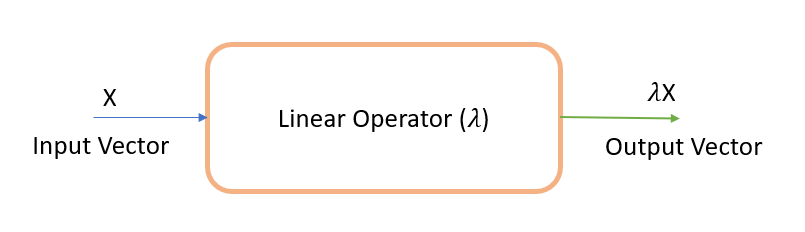
\includegraphics[scale=0.6]{images/eigen-value-vector.png}
\end{figure}
\[AX=\lambda X \Rightarrow AX-\lambda X=0\ \ \ \ \ \ \ (A-\lambda)X=0 \Rightarrow BX=0 \text{ [Homogenous]}\]
\textbf{Characteristic Equation} for Matrix A is given as\\
For 2x2 Matrix, \(\lambda^2-\beta_1\lambda+|A|=0\)\\
For 3x3 Matrix, \(\lambda^3-\beta_1\lambda^2+\beta_2\lambda-|A|=0\)\\
\(\beta_1\rightarrow\text{sum of the diagnol elements(trace); } \beta_2\rightarrow\text{Sum of minors of diagnol elements}\)\vspace{0.2cm}\\
\textbf{Algebric Multiplicity (AM)} of an eigen value\\
If ``\(\lambda\)'' is repeated ``m" times, then AM = m\vspace{0.2cm}\\
\textbf{Geometric Multiplicity (GM)} of an eigen value\\
If ``\(\lambda\)" has ``p" linear independent eigen vectors then GM=p\\
\(GM\ of\ \lambda = n-p(A-\lambda I)=n-r\)
\subsection*{Properties of Eigen Values and Eigen Vectors}
\begin{enumerate}
    \item sum of Eigen Values = trace of the matrix
    \item product of Eigen Values = \(|A|\)
    \item A and \(A^T\) will have same eigen values
    \item The rank of the matrix is equal to the number of non-zero eigen values of the matrix(except triangular matrix)
    \item For a triangular matrix, the eigen values are equal to diagnol elements.
    \item Relation between Eigen Value and Eigen Vector for different form of the given matrix.
    \begin{table}[h!]
    \centering
    \setlength{\tabcolsep}{1em}
    \begin{tabu}{ccc}
    \textbf{Matrix} & \textbf{Eigen Value}               & \textbf{Eigen Vector} \\
    A               & \(\lambda\)                        & X                     \\
    \(A^n\)         & \(\lambda^n\)                      & X                     \\
    A+I             & \(\lambda+I\)                      & X                     \\
    KA              & \(K\lambda\)                       & X                    
    \end{tabu}
    \end{table}
    \item If the sum of elements of every row/column is same then one of the eigen value of the matrix is equal to the sum.
    \item For a real matrix, if \(\alpha+i\beta\) is an eigen value then \(\alpha-i\beta\) will also be an eigen value[conjugate pair].
    \item If a eigen value is \(\alpha+i\beta\) for a complex matrix, then there is no conjugate pair.
    \item The eigen values of a real symmetric matrix are real.
    \item The eigen values of a real skew-symmetric matrix are either zero (or) purely imaginary.
    \item The eigen vector corresponding to the distinct eigen values of a real symmteric matrix will be orthogonal to each other.
    \item The eigen values of a hermition matrix are always real.
    \item The eigen values of a unitary matrix (or) real orthogonal matrix satisfies \(|\lambda|=1\)
    \item The number of linearly independent eigen vectors of a matrix are equal to the number of distinct eigen values of the matrix.
\end{enumerate}


\subsection*{Cayley Hamilton Theorem}
Every square matrix satisfies its own characteristic equation.
\[\lambda^2-(trace)\lambda+|A|=0\ \Rightarrow A^2-(trace)A+|A|=0\]
\pagebreak

% Section
\section{Trignometric Relations}
All the basic and important trignometric relations are listed in this section.

\subsection{Basics}
\textbf{Comman Angles of sin, cos and tan}
\begin{table}[h!]
\centering
\setlength{\tabcolsep}{2em}
\tabulinesep=3.5mm
\begin{tabu}{|c|c|c|c|c|c|}
\hline
\textbf{Degrees} & \textbf{\(0^\circ\)} & \textbf{\(30^\circ\)} & \textbf{\(45^\circ\)} & \textbf{\(60^\circ\)} & \textbf{\(90^\circ\)} \\ \hline
\textbf{Radians} & 0                     & \(\frac{\pi}{6}\)      & \(\frac{\pi}{4}\)      & \(\frac{\pi}{3}\)      & \(\frac{\pi}{2}\)      \\ \hline
\textbf{sin}     & 0                     & \(\frac{1}{2}\)        & \(\frac{1}{\sqrt{2}}\) & \(\frac{\sqrt{3}}{2}\) & 1                      \\ \hline
\textbf{cos}     & 1                     & \(\frac{\sqrt{3}}{2}\) & \(\frac{1}{\sqrt{2}}\) & \(\frac{1}{2}\)        & 0                      \\ \hline
\textbf{tan}     & 0                     & \(\frac{1}{\sqrt{3}}\) & 1                      & \(\sqrt{3}\)           & \(\infty\)             \\ \hline

\end{tabu}
\end{table}
\textbf{Reciprocal Functions}
\[csc\ x=\frac{1}{sin\ x}\ \ \ \ \ \ \ sec\ x=\frac{1}{cos\ x}\ \ \ \ \ \ \ cot\ x=\frac{1}{tan\ x} \]
\textbf{Even/Odd Relation}
\[sin\ (-x)=-sin\ x\ \ \ \ \ \ \ cos\ (-x)=cos\ x\ \ \ \ \ \ \ tan\ (-x)=-tan\ x\]


\subsection{Identities}
\textbf{Pythagorous Identities}
\[sin^2x+cos^2x=1\ \ \ \ \ \ \ 1+cot^2x=csc^2x\ \ \ \ \ \ \ 1+tan^2x=sec^2x\]
\textbf{Cofunction Identities}
\begin{align*}
    \sin(\frac{\pi}{2} - x) &= \cos x\hspace{3cm}
    \cos(\frac{\pi}{2} - x) &= \sin x\hspace{3cm}
    \tan(\frac{\pi}{2} - x) &= \cot x\\
    \cot(\frac{\pi}{2} - x) &= \tan x\hspace{3cm}
    \sec(\frac{\pi}{2} - x) &= \csc x\hspace{3cm}
    \csc(\frac{\pi}{2} - x) &= \sec x
\end{align*}

\subsection{Angular Relations}
\textbf{Sum and Difference of Angles}
\begin{align*}
    \sin(x + y) = \sin x \cos y + \cos x \sin y\hspace{2cm}
    \sin(x - y) = \sin x \cos y - \cos x \sin y\\
    \cos(x + y) = \cos x \cos y - \sin x \sin y\hspace{2cm}
    \cos(x - y) = \cos x \cos y + \sin x \sin y\\
    \tan(x + y) = \frac{\tan x + \tan y}{1 - \tan x \tan y}\hspace{4cm}
    \tan(x - y) = \frac{\tan x - \tan y}{1 + \tan x \tan y}
\end{align*}

\textbf{Dobule Angles}
\begin{align*}
    \sin(2x)  &= 2 \sin x \cos x\\
    \cos(2x)  &= \cos^2 x - \sin^2 x = 2 \cos^2 x - 1 = 1 - 2 \sin^2 x\\
    \tan(2x)  &= \frac{2 \tan x}{1 - \tan^2 x}
\end{align*}
\textbf{Half Angles}
\begin{align*}
    \sin \frac{x}{2}  = \pm \sqrt{ \frac{1 - \cos x }{2} }\hspace{2cm}
    \cos \frac{x}{2}  = \pm \sqrt{ \frac{1 + \cos x }{2} }
\end{align*}
\begin{align*}
    \tan \frac{x}{2}  = \frac{1 - \cos x }{\sin x}= \frac{ \sin x }{ 1 + \cos x }
\end{align*}

\subsection{sum, Power and Products Relations}
\textbf{Power Reducing Formulas}
\begin{align*}
  \sin^2 x  = \frac{1 - \cos 2x}{2}\hspace{2cm}
  \cos^2 x  = \frac{1 + \cos 2x}{2}\hspace{2cm}
  \tan^2 x  = \frac{1 - \cos 2x}{1 + \cos 2x}
\end{align*}
\textbf{Product to sum}
\begin{align*}
  \sin x \sin y &= \frac{1}{2}\big[\cos(x - y) - \cos(x + y)\big]\\
  \cos x \cos y &= \frac{1}{2}\big[\cos(x - y) + \cos(x + y)\big]\\
  \sin x \cos y &= \frac{1}{2}\big[\sin(x + y) + \sin(x - y)\big]\\
  \tan x \tan y &= \frac{ \tan x + \tan y }{ \cot x + \cot y }\\
  \tan x \cot y &= \frac{ \tan x + \cot y }{ \cot x + \tan y }
\end{align*}
\textbf{Sum to Product}
\begin{align*}
  \sin x + \sin y &= 2 \sin \Big( \frac{x + y}{2} \Big) \cos \Big( \frac{x - y}{2} \Big)\\
  \sin x - \sin y &= 2 \cos \Big( \frac{x + y}{2} \Big) \sin \Big( \frac{x - y}{2} \Big)\\
  \cos x + \cos y &= 2 \cos \Big( \frac{x + y}{2} \Big) \cos \Big( \frac{x - y}{2} \Big)\\
  \cos x - \cos y &= -2 \sin \Big( \frac{x + y}{2} \Big) \sin \Big( \frac{x - y}{2} \Big)\\
  \tan x + \tan y &= \frac{ \sin(x + y) }{ \cos x \cos y}\\
  \tan x - \tan y &= \frac{ \sin(x - y) }{ \cos x \cos y}\\
\end{align*}
\pagebreak

% Section
\section{Differentiation Formulas}
\begin{multicols}{2}
\begin{enumerate}
    \item \(\frac{d}{dx}k=0\)
    \item \(\frac{d}{dx}f(g(x))=f'(g(x)).g'(x)\)
    \item \(\frac{d}{dx}[f(x)g(x)]=f(x)g'(x)+g'(x)f(x)\) % 3
    \item \(\frac{d}{dx}x^n=nx^{n-1}\)
    \item \(\frac{d}{dx}e^x=e^x\)
    \item \(\frac{d}{dx}sin\ x=cos\ x\)
    \item \(\frac{d}{dx}tan\ x=sec^2\ x\)
    \item \(\frac{d}{dx}sec\ x=sec\ x\ tan\ x\)
    \item \(\frac{d}{dx}\ sin^{-1}x=\frac{1}{\sqrt{1-x^2}}\)
    \item \(\frac{d}{dx}\ tan^{-1}x=\frac{1}{\sqrt{x^2+1}}\)
    \item \(\frac{d}{dx}\ sec^{-1}x=\frac{1}{|x|\sqrt{x^2-1}}\)
    \item \(\frac{d}{dx}[k(f(x)]=k.f'(x)\) % 12
    \item \(\frac{d}{dx}=[f(x)\pm g(x)]=f'(x)\pm g'(x)\) % 13
    \item \(\frac{d}{dx}\left(\frac{f(x)}{g(x)}\right)=\frac{g(x)f'(x)-f(x)g'(x)}{[g(x)]^2}\)
    \item \(\frac{d}{dx}\ ln|x|=\frac{1}{x}; \frac{d}{dx}\ log_a|x|=\frac{1}{x ln a} \)
    \item \(\frac{d}{dx}a^x=a^x\ ln\ a\)
    \item \(\frac{d}{dx}cos\ x=-sin\ x\)
    \item \(\frac{d}{dx}cot\ x=-csc^2\ x\)
    \item \(\frac{d}{dx}csc\ x=-csc\ x\ cot\ x\)
    \item \(\frac{d}{dx}\ cos^{-1}x=\frac{-1}{\sqrt{1-x^2}}\)
    \item \(\frac{d}{dx}\ cot^{-1}x=\frac{-1}{\sqrt{x^2+1}}\)
    \item \(\frac{d}{dx}\ csc^{-1}x=\frac{-1}{|x|\sqrt{x^2-1}}\)
\end{enumerate}
\end{multicols}


% Section 
\section{Integration Formulas}
\begin{multicols}{2}
\begin{enumerate}
    \item \(\int \ dx=x+C\) %1
    \item \(\int \frac{dx}{x}=ln|x|+C\) % 2
    \item \(\int e^x \ dx=e^x+C\) % 3
    \item \(\int \frac{f'(x)}{f(x)}\ dx=ln(f(x))+C\) % 4
    \item \(\int sin\ x\ dx=-cos\ x+C\) % 5
    \item \(\int tan\ x\ dx=-ln|cos\ x|=ln|sec\ x|\ +C\) % 6
    \item \(\int sec\ x\ dx=ln|sec\ x+tan\ x|+C\) % 7
    \item \(\int sec\ x\ tan\ x\ dx=sec\ x+C\) % 8
    \item \(\int \frac{dx}{\sqrt{a^2-x^2}}=sin^{-1}\frac{x}{a}+C\) % 9
    \item \(\int \frac{dx}{x\sqrt{x^2-a^2}}=\frac{1}{a}sec^{-1}\frac{|x|}{a}+C\) %10
    \item \(\int x^n\ dx=\frac{x^{n+1}}{n+1}+C\) % 11
    \item \(\int a^x\ dx=\frac{1}{ln\ a} a^x+C\) % 12
    \item \(\int ln\ x\ dx=x\ ln\ x-x+C\) % 13
    \item \(\int \frac{f'(x)}{\sqrt{f(x)}}\ dx=2\sqrt{f(x)}+C\) % 14
    \item \(\int cos\ x\ dx=sin\ x+C\) % 15
    \item \(\int cot\ x\ dx=ln|sin\ x|=-ln|csc\ x|\ +C\) % 16
    \item \(\int csc\ x\ dx=-ln|csc\ x+cot\ x|+C\) % 17
    \item \(\int csc\ x\ cot\ x\ dx=-csc\ x+C\) % 18
    \item \(\int \frac{dx}{a^2+x^2}=\frac{1}{a}tan^{-1}\frac{x}{a}+C\) %19
    \item \(\int_0^{\infty}cos^2x\ dx=\int_0^{\infty}sin^2x\ dx=\frac{1}{2}\sqrt{\frac{\pi}{2}}\) %20
\end{enumerate}
\end{multicols}

\textbf{Integration by Parts} \(\int u\ dv = uv_1 - u'\int v_2\) where \(v^n\) stands for integrating the given function n times. [priority for u - ILATE]


% Section 2
\chapter*{Calculus}
\section{Calculus}

\subsection{Limit, Continuity \& Differentiability}
\textbf{Conditions for Continuvity} \vspace{0.2cm} \\
f(x) is continuous at point x = a, if
\begin{enumerate}
    \item \(\lim_{x\to a^-} f(x)=\lim_{x\to a^+} f(x) \) (LHL=RHL)
    \item f(a) is finite
    \item \(\lim_{x\to a^-} f(x)=\lim_{x\to a^+} f(x) =f(a)\)
\end{enumerate}
\textbf{Conditions for Differentiability} \vspace{0.2cm} \\
f(x) is differentiable at point x=a, if
\begin{enumerate}
    \item f(x) should be continuous
    \item \(\lim_{h\to0^-}\frac{f(x+h)-f(x)}{h}=\lim_{h\to0^+}\frac{(x+h)-f(x)}{h}\) (LHD=RHD)
    \item f(x) should not have vertical tangent at x=0
\end{enumerate}
\textbf{Key Points}
\begin{enumerate}
    \item The derivative at any point on the curve given the value of the slope of the tangent to the curve at that point.
    \item \(sinx,\ cosx,\ e^x\) and polynomial functions are always continuous \& differentiable.
    \item \(lnx\) is continuous and differentiable \(\forall x>0\)
    \item If f(x) and g(x) are continuous and differentiable functions then the following function will also be continuous and differentiable.
        \(i) f(x) \pm g(x) \ \ ii) f(x)g(x) \ \ iii) \frac{f(x)}{g(x)}, g(x) \neq 0\)
    \item sharp (or) edge (or) break point is the point in which the nature of the curve changes(sudden change in slope). If a function is continuous at a point but RHD \( \neq \) LHD, then we get a sharp point.
    \item \(|x-a|\) is continuous but not differentiable at x = a.
\end{enumerate}

\subsection*{Applying Limit to f(x)}
\[\lim_{x \to a} f(x) = k\]
\textbf{L'Hospital Rule} if Applying a limit in f(x) results \(\frac{0}{0}\ or\ \frac{\infty}{\infty}\), then differentiate numerator and denominator, continue differntiating and applying limits till the results not infinite.\\
If Applying Limits in f(x) results in \(\infty - \infty\), then substitution method is used. Choose a substitution value in such a way a limit is not infinity.

\subsection{Mean Value Theorems}
\textbf{Lagrange's Mean Value Theorem}\vspace{0.2cm}\\
If f(x) be a real valued function such that \\
1. It is continuous in [a, b] 2. It is differentiable in (a, b) \\
Then there exists a point \(x = C \in (a, b) \) such that
\[f'(c)= \frac{f(b)-f(a)}{b-a}\]
\textbf{Rolle's Theorem}\vspace{0.2cm}\\
If f(x) be a real valued function such that \\
1. It is continuous in [a, b] 2. It is differentiable in (a, b) 3. f(a) = f(b)\\
Then there exists a point \(x = C \in (a, b) \) such that
\[f'(c)=0\] 
\textbf{Cauchy's Mean Value Theorem}\vspace{0.2cm}\\
If f(x) and g(x) be two real valued functions such that\\
1. It is continuous in [a, b] 2. differntiable in (a, b)\\
Then there exists a point \(x = C \in (a, b) \) such that
\[\frac{f'(c)}{g'(c)}=\frac{f(b)-f(a)}{g(b)-g(a)}\]

\subsection*{Increasing and Decreasing Functions}
A function is said to be increasing if \(f'(x) > 0\).\\
A function is said to be decreasing if \(f'(x) < 0\).
\begin{figure}[h!]
    \centering
    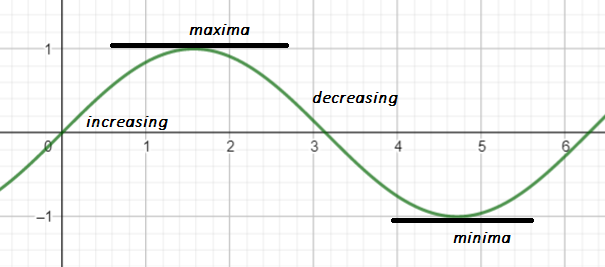
\includegraphics[scale=0.775]{images/max-min.png}
\end{figure}

\subsection{Maxima and Minima}
For any function f(x) the tangent to local maxima and local minima is always parallel to x-axis, then f'(x) = 0 gives the stationary points.\\
Determine the maxima and minima for the given function using the below methods.\\
\textbf{1st Derivative Test}
\begin{enumerate}
    \item Calculate the stationary point using the equation f'(x) = 0
    \item If the point around the 1st derivative changes its sign from +ve to -ve then that stationary point is a point of local maxima.
    \item If the point around the 1st derivative changes its sign from -ve to +ve then that stationary point is a point of local minima.
\end{enumerate}
\textbf{2nd Derivative Test}
\begin{enumerate}
    \item Calculate the stationary point by the equation f'(x) = 0
    \item let x=x0 be the stationary point.\vspace{0.2cm}\\
    \( f''(x)_{x=x_0} = 
    \begin{cases}
        +ve, & minima\\
        0,   & go further\\
        -ve, & maxima
    \end{cases} \)\hspace{1cm}
    \( f^{iv}(x)_{x=x_0} = 
    \begin{cases}
        +ve, & minima\\
        0,   & go further\\
        -ve, & maxima
    \end{cases} \)\vspace{0.2cm}\\
    \( f'''(x)_{x=x_0} = 
    \begin{cases}
        +ve, & \text{neither maximum or minimum}\\
        0,   & \text{go further}\\
        -ve, & \text{neither maximum or minimum}
    \end{cases} \)
\end{enumerate}
\textbf{Inflation Point} - stationary point at which the curve will be increasing/decreasing before and after stationary points then it known as point of inflation.

\subsection*{Wavy Curve Method}
Easy method to find maxima and minima but only applicable to f'(x) having polynomial inequalities.\\
Wavy Curve always start from right at positive and then change sign for every different roots.
\begin{figure}[h!]
    \centering
    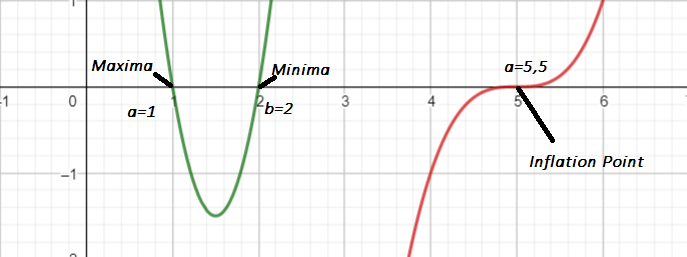
\includegraphics[width=\linewidth]{images/wavy-curve.png}
\end{figure}

\subsection*{Global Maxima and Minima}
For a function f(x) in [a, b] global maxima and minima can be determined by
\begin{enumerate}
    \item Find stationary points f'(x) = 0
    \item find the values of \(f(a), f(b), f(x_n)\) and then compare the values to get maxima and minima.
\end{enumerate}
\textbf{Important Note:}
\begin{enumerate}
    \item If interval not mentioned then find local maxima and local minima else find global maxima and global minima.
    \item No of Stationary Point \(\alpha\) No of Maxima and minima.
    \item If No of stationary point is 1 then local maxima/minima is global maxima/minima.
\end{enumerate}


\subsection{Partial Differentiation}
\begin{enumerate}
    \item For a function of single independent variable, simple or ordinary derivative will exist.
    \[y=f(x)=\frac{dy}{dx} \]
    \item For a function of more than one independent variable partial derivative will exist.
    \[u=f(x,y),\ \frac{\partial u}{\partial x},\ \frac{\partial u}{\partial y}\]
    \item The number of partial derivatives existing for a functional relation is exactly equal to the number of independent variables.
    \item The procedure to evaluate partial derivatives is same as that of the simple derivatives but the only difference is that all other independent variable will remain constant.
    \item Dependent variable should never be assumed constant. 
\end{enumerate}

\subsection*{Conditions for Maxima and Minima for Paritial Derivaties}
Let f(x, y) be any two functions of variables x and y, then
\[r=\frac{\partial^2f}{\partial x^2},\ \ s=\frac{\partial^2f}{\partial x\partial y}, \ \ t = \frac{\partial^2f}{\partial y^2}\]
\begin{enumerate}
    \item if \(rt-s^2>0;\ r<0,\ t<0,\) then the point is local maxima
    \item if \(rt-s^2>0;\ r>0,\ t>0,\) then the point is local minima
    \item if \(rt-s^2<0;\) Neither Maxima or Minima
    \item if \(rt-s^2=0;\ r<0,\ t<0,\) No conclusion further investigation required.
\end{enumerate}
\textbf{Homogeneous Function}\\
A function having same degree in all its terms is called Homogeneous function. A homogeneous function can be expressed either as a function of `y/x' or as a function of ``x/y''.
\[f(x, y)=x^nF(x/y)\  (or)\ x^n F(y/x) \]
\subsection*{Euler's Theorem for Homogeneous function}
\begin{fleqn}
\textbf{Corallory 0:} If u=f(x,y) be a homogeneous function of degree n.
\[1.\ x\frac{\partial u}{\partial x} + y\frac{\partial u}{\partial y}=nu\ \ \ \ \ \ \
  2.\ x^2\frac{\partial^2 u}{\partial x^2} + y^2\frac{\partial^2 u}{\partial y^2} + 2xy\frac{\partial^2u}{\partial x\partial y}=n(n-1)u \]
\textbf{Corallory 1:} If u is not a homogeneous function but f(u) is a homogeneous function of degree n.
\[1.\ x\frac{\partial u}{\partial x} + y\frac{\partial u}{\partial y}=\frac{nf(u)}{f'(u)}= g(u) \ \ \ \ \ \ \
  2.\ x^2\frac{\partial^2 u}{\partial x^2} + y^2\frac{\partial^2 u}{\partial y^2} + 2xy\frac{\partial^2u}{\partial x\partial y}=g(u)[g'(u)-1] \]
\textbf{Corallory 2:} If u=f(x,y) + g(x,y) + h(x,y) where f, g, h are homogeneous function of degree m, n, p respectively, then.
\[1.\ x\frac{\partial u}{\partial x} + y\frac{\partial u}{\partial y}=mf+ng+ph\ \ \ \ \ \ \
  2.\ x^2\frac{\partial^2 u}{\partial x^2} + y^2\frac{\partial^2 u}{\partial y^2} + 2xy\frac{\partial^2u}{\partial x\partial y}=m(m-1)f+n(n-1)g+p(p-1)h \]
\end{fleqn}


\subsection{Total Derivatives}
\begin{enumerate}
    \item In a composite relation, the derivative of an initial variable w.r.t final variable is called as Total derivative.
    \item The number of total derivatives existing for a composite relation is exactly equal to the number of final variables.
    \item The number of terms present in the expression of a total derivative is exactly equal to the number of intermediate variables.
    \[w\rightarrow x,y\rightarrow t\ \  \frac{dw}{dt}=\frac{\partial w}{\partial x}\frac{dx}{dt}+ \frac{\partial w}{\partial y}\frac{dy}{dt}\]
\end{enumerate}

\subsection*{Taylor Series}
If f(X) has all its derivative as finite and contiuous \(\forall x \)
\[f(x) = f(a) + hf'(a)+h^2f''(a)+h^3f'''(a)+\ldots\ldots.\infty\]
If f(x,y) has all its derivative as finite and continuous at all point(x,y)
\begin{multline*}
f(x+h, y+k)=f(x,y)+[hf_x+kf_y]+\frac{1}{2!}[h^2f_{xx}+k^2f_{yy}+2hkf_{xy}] \\
+\frac{1}{3!}[h^3f_{xxx}+k^3f_{yyy}+3hk^2f_{xyy}+3h^2kf_{xxy}] + \ldots
\end{multline*}

\subsection{Gamma Function}
\begin{fleqn}
\[\Gamma n = \int_{0}^{\infty} e^{-x} x^{n-1} \,dx\ \ \ \ \ \ 
\frac{\Gamma n}{k^n}=\int_{0}^{\infty} e^{-kx} x^{n-1} \,dx\]
\[\Gamma \frac{1}{2} = \sqrt{\pi}\ \ \ \ \ \ \Gamma n\ \Gamma(1-n)=\frac{\pi}{sin\ n\pi}
\ \ \ \  \Gamma (n+1) = 
\begin{cases}
    n\sqrt{n} & \text{'n' is fraction}\\
    n! & \text{'n' is integer}
\end{cases}
\]
\end{fleqn}

\subsection{Beta Function}
\begin{fleqn}
\[\beta(m,n)=\int_{0}^{1} x^{m-1} (1-x)^{n-1} \,dx\ \ \ \ \ 
\beta(m, n)=\int_{0}^{\infty}\frac{x^{n-1}}{(1+x)^{m+n}} \,dx\]
\[\beta(m,n)=\beta(n,m)\ \ \ \ \ \ \beta(m,n)=\frac{\Gamma m\ \Gamma n}{\Gamma (m+n)}\ \ \ \
\frac{1}{2}\beta\left(\frac{p+1}{2}, \frac{q+1}{2} \right)=\int_{0}^{\pi/2}sin^p\theta\ cos^q\theta \,d\theta\]
\textbf{Points to Remember}\\
\(1. \int_0^a f(x) \,dx = 
    \begin{cases}
    0 & \text{if f(a-x)=-f(x)}\\
    2\int_0^{a/2}f(x) \,dx & \text{if f(a-x)=f(x)}
    \end{cases}
\)            
\(2. \int_{-a}^a f(x) \,dx = 
    \begin{cases}
    0 & \text{if f(x) is odd}\\
    2\int_0^{a}f(x) \,dx & \text{if f(x) is even}
    \end{cases}
\)
\end{fleqn}

\subsection{Double and Triple Integrals}
In Double and Triple Integrals, we need to find the limits of the function with respect to x, y and z-axis based on the given equation. To do that use the given equations in the problem.\\
1. Find the intersection point and plot the graph.\\
2. Draw a strip parallel to x-axis or y-axis based on the integration order.\\
3. Now, use sliding approach on the parallel axis to obtain limits for the constant set and find the limits for variable set using the strip and the equation of the given curve.\\
\begin{table}[h!]
\centering
\setlength{\tabcolsep}{1em}
\tabulinesep=1.5mm
\begin{tabu}{llll}
0 & a & Constant Set & \(||el\ to\ y-axis\) \\
0 & x & Variable Set & First Priority
\end{tabu}
\end{table}
\begin{figure}[h!]
    \centering
    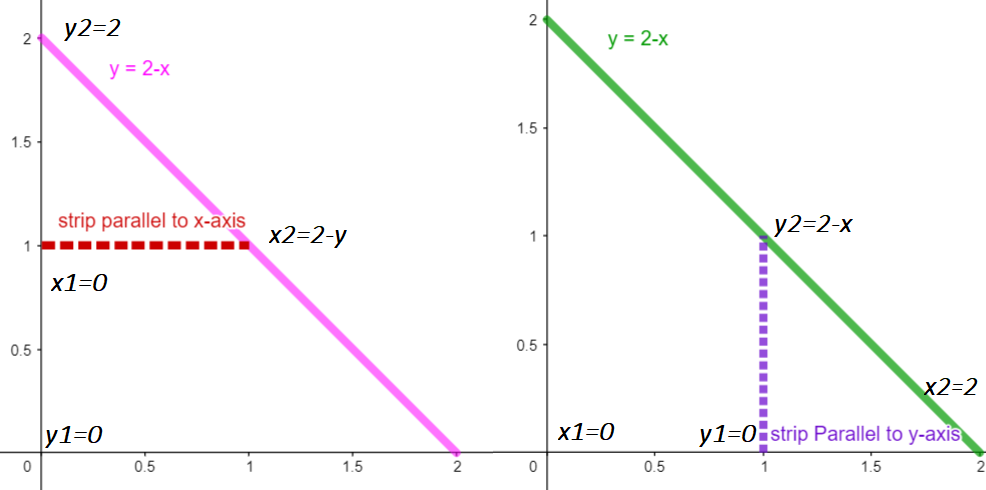
\includegraphics[scale=0.6]{images/limit-finder.png}
\end{figure}


\subsection{Fourier Series}
\textbf{Periodic Function} - A function f(x) is periodic function of period \(T(T>0)\ if\ f(x)=f(x+T) \forall x\)\vspace{0.2cm}\\
\textbf{Orthogonal Function} - Two non-zero function f(x) and g(x) are said to be orthogonal on \(a \leq x \leq b\) if,
\[\int_a^bf(x)g(x)dx=0\]

\subsection*{Dirichlet's Condition}
The fourier series f(x) converges if
\begin{enumerate}
    \item f(x) is periodic, single values and finite.
    \item The function f(x) has finite number of finite discontinuties in any one period.
    \item The function f(x) must have finite number of maxima and minima.
\end{enumerate}

\subsection*{Fourier Series}
The fourier series of a periodic function f(x) of period 2L on the interval (-L, L) is defined as
\[f(x)=\frac{a_0}{2}+\sum_{n=1}^{\infty}\left(a_n cos\frac{n\pi x}{L}+b_nsin \frac{n\pi x}{L}\right)\]
\[a_0=\frac{1}{L}\int_{-L}^Lf(x)dx\ \ \ \ a_n=\frac{1}{L}\int_{-L}^Lf(x)cos\frac{n\pi x}{L}\ dx\ \ \ \ b_n = \frac{1}{L}\int_{-L}^Lf(x)sin\frac{n\pi x}{L}\ dx\]
The fourier series of periodic function f(x) of period 2\(\pi\) on the interval \((-\pi, \pi)\) is defined as
\[f(x)=\frac{a_0}{2}+\sum_{n=1}^{\infty}\left(a_n cosnx+b_nsinnx\right)\]
\[a_0=\frac{1}{\pi}\int_{-\pi}^{\pi}f(x)dx\ \ \ \ a_n=\frac{1}{\pi}\int_{-\pi}^{\pi}f(x)cosnx\ dx\ \ \ \ b_n = \frac{1}{\pi}\int_{-\pi}^{\pi}f(x)sinnx\ dx\]
\textbf{Note: }Fourier Series expressing given function f(x) in terms of cos \& sin functions.\vspace{0.2cm}\\
\textbf{Example:} Fourier series of \(sinx-sin3x+cos2x\ in\ [-\pi, \pi]\ is\)\vspace{0.3cm}\\
The given function is itself a fourier series.\vspace{0.2cm}\\
The values of \(a_0 = 0, a_1=0, a_2=1\) and \(b_1=1, b_2=0, b_3=-1\)

\subsection*{Convergence of Fourier Series}
\begin{itemize}
    \item If f(x) is continuous at x=c; \([Fourier\ Series\ of\ f(X)]_{x=c}=f(c)\)
    \item If f(x) is not continuous at x=c; \([Fourier\ Series\ of\ f(X)]_{x=c}= \frac{f(c^-)+f(c^+)}{2}\)
\end{itemize}

\subsection*{Parseval Identity}
The parseval identity for fourier series in the interval (c,c+2l) is defined as
\[\frac{1}{2l}\int_c^{c+2l}[f(x)]^2=\frac{a_0^2}{4}+\frac{1}{2}\sum_{n=1}^{\infty}\left[a_n^2+b_n^2\right]\]
\textbf{Even Function} - f(-x) = f(x) then the graph of y=f(x) is symmetric about y-axis.\vspace{0.3cm}\\
\textbf{Odd Function} - f(-x) = -f(x) then the graph of y=f(x) is symmetric about origin.\vspace{0.3cm}\\
Parseval identity is used to derive standard series formula from fourier series.\\

\subsection*{Important Results}
\begin{multicols}{2}
\begin{itemize}[label={}]
    \item \[\frac{1}{1^2}+\frac{1}{2^2}+\frac{1}{3^2}+\frac{1}{4^2}+\ldots\ldots.=\frac{\pi^2}{6}\]
    \item \[\frac{1}{1^2}+\frac{1}{3^2}+\frac{1}{5^2}+\frac{1}{7^2}+\ldots\ldots.=\frac{\pi^2}{8}\]
    \item \[\frac{1}{2^2}+\frac{1}{4^2}+\frac{1}{6^2}+\frac{1}{8^2}+\ldots\ldots.=\frac{\pi^2}{24}\]
    \item \[\frac{1}{1^4}+\frac{1}{2^4}+\frac{1}{3^4}+\frac{1}{4^4}+\ldots\ldots.=\frac{\pi^2}{90}\]
    \item \[1-\frac{1}{3}+\frac{1}{5}-\frac{1}{7}+\ldots\ldots\ldots.=\frac{\pi}{4}\]
\end{itemize}
\end{multicols}

\subsection*{Fourier Cosine Series}
The Fourier series of Even periodic function f(x) of period \(2\pi\) on the interval \(-\pi, \pi\) is fourier cosine series.
\[f(x)=a_0+\sum_{n=1}^{\infty}a_n cosnx\ \ \ \ \ a_0=\frac{2}{\pi}\int_0^{\pi}f(x)\ dx\ \ \ \ \ a_n=\frac{2}{\pi}\int_0^{\pi}f(x)cosnx\ dx\]

\subsection*{Fourier Sine Series}
The Fourier series of Odd periodic function f(x) of period \(2\pi\) on the interval \(-\pi, \pi\) is fourier sine series.
\[f(x)=\sum_{n=1}^{\infty}b_n sinnx\ \ \ \ \ b_n=\frac{2}{\pi}\int_0^{\pi}f(x)sinnx\ dx\]


\subsection*{Half Range Fourier Series}
\textbf{Half Range Cosine Series} - It is defined in the interval \((0, \pi)\)
\[f(x)=a_0+\sum_{n=1}^{\infty}a_n cosnx\ \ \ \ \ a_0=\frac{2}{\pi}\int_0^{\pi}f(x)\ dx\ \ \ \ \ a_n=\frac{2}{\pi}\int_0^{\pi}f(x)cosnx\ dx\]
\textbf{Half Range Sine Series} - It is defined in the interval \((0, \pi)\)
\[f(x)=\sum_{n=1}^{\infty}b_n sinnx\ \ \ \ \ b_n=\frac{2}{\pi}\int_0^{\pi}f(x)sinnx\ dx\]


\subsection{Gradient, Divergence and Curl}
\textbf{Vector Differential Operator} 
 also known as Del Operator is given by
\[\overrightarrow{\rm \nabla} = \overrightarrow{\rm i}\frac{\partial}{\partial x} + 
           \overrightarrow{\rm j}\frac{\partial}{\partial y} + 
           \overrightarrow{\rm k}\frac{\partial}{\partial z}\]
\textbf{Gradient} is a vector quantity and it is defined as \\
\[Gradient(\emptyset) = \overrightarrow{\rm \nabla}\emptyset = 
        \overrightarrow{\rm i}\frac{\partial\emptyset}{\partial x} + 
        \overrightarrow{\rm j}\frac{\partial\emptyset}{\partial y} + 
        \overrightarrow{\rm k}\frac{\partial\emptyset}{\partial z}\]
\(Let\ \overrightarrow{\rm F} = F_x\overrightarrow{\rm i}+F_y\overrightarrow{\rm j}
+F_z\overrightarrow{\rm F}\)\\
\textbf{Divergence} is a scalar quantity and it is defined as \\
\[Divergence\overrightarrow{\rm F}=\overrightarrow{\rm \nabla}\ \overrightarrow{\rm F} = 
\frac{\partial}{\partial x}F_x + \frac{\partial}{\partial y}F_y +
\frac{\partial}{\partial z}F_z\]
\textbf{Curl} is a vector quantity and it is defined as \\
\[Curl\overrightarrow{\rm F}=|\overrightarrow{\rm \nabla} \times \overrightarrow{\rm F}| =
\begin{vmatrix}
\overrightarrow{\rm i} & \overrightarrow{\rm j} & \overrightarrow{\rm k}\\ 
\frac{\partial}{\partial x} & \frac{\partial}{\partial y} & \frac{\partial}{\partial z} \\
F_x & F_y & F_z
\end{vmatrix}
\]

\subsection*{Properties}
\begin{enumerate}
    \item \(\overrightarrow{\rm \nabla}^2\) is known as Laplacian Operator and it is defined as below
    \[\overrightarrow{\rm \nabla}.(\overrightarrow{\rm \nabla}\emptyset) = \frac{\partial^2 \emptyset}{\partial x^2} + \frac{\partial^2 \emptyset}{\partial y^2} + \frac{\partial^2 \emptyset}{\partial z^2}\]
    \item \(\overrightarrow{\rm \nabla}\times(\overrightarrow{\rm \nabla}\emptyset) = 0,\ \ \ \ \ \overrightarrow{\rm \nabla}\times\overrightarrow{\rm \nabla}=0\)
    \item \(\overrightarrow{\rm \nabla}.(\overrightarrow{\rm \nabla}\times\overrightarrow{\rm F} = 0)\)
    \item \(\overrightarrow{\rm \nabla}\times(\overrightarrow{\rm \nabla}\times\overrightarrow{\rm F})=\overrightarrow{\rm \nabla}.(\overrightarrow{\rm \nabla}.\overrightarrow{\rm F})-\overrightarrow{\rm \nabla}^2\overrightarrow{\rm F}\)
\end{enumerate}

\subsection*{Important Results}
\begin{itemize}
    \item Directional Derivative = \(\overrightarrow{\rm \nabla}.\emptyset\ \hat{a}\ \ \ \ \ \hat{a}=\left[ \frac{\overrightarrow{\rm a}}{|\overrightarrow{\rm a}|} \right]\ \ \ \ \ |\overrightarrow{\rm a}|=\sqrt{a^2 + b^2 + c^2} \)
    \item Curl \(\overrightarrow{\rm F} = 0\) means it is irrotational.
    \item Divergence \(\overrightarrow{\rm F} = 0\) means it is solenoidal
    \item Angle between two planes is given by
    \(cos\theta = \frac{\overrightarrow{\rm \nabla} f1. \overrightarrow{\rm \nabla} f2}{|\overrightarrow{\rm \nabla} f1|.|\overrightarrow{\rm \nabla} f2|}\)
    \item Two planes are said to be orthogonal if, \(\overrightarrow{\rm \nabla} f1. \overrightarrow{\rm \nabla} f2 = 0\)
\end{itemize}

\subsection*{Vector Identities}
\begin{enumerate}
    \item \(\overrightarrow{\rm \nabla}(f+g)=\overrightarrow{\rm \nabla} f +\overrightarrow{\rm \nabla} g,\)\hspace{1cm}\(\overrightarrow{\rm \nabla}(\overrightarrow{\rm A}+\overrightarrow{\rm B}) = \overrightarrow{\rm \nabla}\overrightarrow{\rm A}+ \overrightarrow{\rm \nabla}\overrightarrow{\rm B},\)\hspace{1cm} \(\overrightarrow{\rm \nabla}\times(\overrightarrow{\rm A}+\overrightarrow{\rm B})=\overrightarrow{\rm \nabla}\times\overrightarrow{\rm A}+\overrightarrow{\rm \nabla}\times\overrightarrow{\rm B}\)
    \item \(\overrightarrow{\rm \nabla}(f.g) = f(\overrightarrow{\rm \nabla} g) + g(\overrightarrow{\rm \nabla} f)\),\hspace{1cm}  \(\overrightarrow{\rm \nabla}(f\overrightarrow{\rm A})=f(\overrightarrow{\rm \nabla} \overrightarrow{\rm A})+\overrightarrow{\rm A}(\overrightarrow{\rm \nabla}.f)\) \hspace{1cm}
    \item  \(\overrightarrow{\rm \nabla}\times(f\overrightarrow{\rm A})=f(\overrightarrow{\rm \nabla}\times\overrightarrow{\rm A})+\overrightarrow{\rm A}\times(\overrightarrow{\rm \nabla}.f)\), \hspace{1cm} \(\overrightarrow{\rm \nabla}(\overrightarrow{\rm A}\times\overrightarrow{\rm B})=\overrightarrow{\rm B}(\overrightarrow{\rm \nabla}\times\overrightarrow{\rm A})-\overrightarrow{\rm A}(\overrightarrow{\rm \nabla}\times\overrightarrow{\rm B})\)
    \item \(\overrightarrow{\rm A}.(\overrightarrow{\rm B}\times\overrightarrow{\rm C})=
    \begin{vmatrix} A_x & A_y & A_z \\ B_x & B_y & B_z \\ C_x & C_y & C_z \end{vmatrix}
    \)
\end{enumerate}
\textbf{\large{Line Integral}} An integration evaluated along the given curve/line.
\[\overrightarrow{\rm F} = F_1\overrightarrow{\rm i}+F_2\overrightarrow{\rm j}+F_3\overrightarrow{\rm k}\ \ \ \ \overrightarrow{\rm dr}=dx\overrightarrow{\rm i}+dy\overrightarrow{\rm j}+dz\overrightarrow{\rm k}\]
\[\oint_C\overrightarrow{\rm F}\overrightarrow{\rm dr}=\oint_CF_1dx+F_2dy+F_3dz\]
If a Multi Variable function is given, then equate it to single variable function using the given equation/curve/points/parameters. Then the Limit will be fixed to 0 to 1
\[Ex:\ x=y=z=t\ \ \  dx=dy=dz=t\ \ \ \oint_C\overrightarrow{\rm F}\overrightarrow{\rm dr}=\int_Cf(x)t \,dt \]
\textbf{\large Surface Integral} An integration evaluated along the given surface by projecting the give surface to xy, yz, zx plane.
Consider \(\emptyset\) as given equation of the surface plane. Then the surface integral is defined as
\[\iint_S\overrightarrow{\rm F}.\hat{n}\,ds\ where\ \hat{n}= \frac{\overrightarrow{\rm \nabla}\emptyset}{|\overrightarrow{\rm \nabla}\emptyset|} \]
Consider if the surface is projected to x-y plane, then the surface integral is given as
\[\iint_S\overrightarrow{\rm F}.\hat{n}\,ds=\iint_R\overrightarrow{\rm F}.\hat{n}\,\frac{dxdy}{|\overrightarrow{\rm n}.\overrightarrow{\rm k}|}\]
\textbf{\large Volume Integral} An integral evaluated over a volume bounded by the surface.
\[\iiint_v F(x,y,z) \, dx\, dy\, dz\]
\subsection{Vector Calculus Theorems}
\subsection*{Green's Theorem}
If R is a closed Region of the XY plane bounded by a simple curve C is given as
\[\int_C(Mdx+Ndy)=\iint_R\left(\frac{\partial N}{\partial x}-\frac{\partial M}{\partial y} \,dxdy \right)\]

\subsection*{Gauss Divergence Theorem}
If a closed surface S bounding a Volume is given by the Gauss Divergence Theorem as below.
\[\oint\oint_S\overrightarrow{\rm F}.\hat{n}\,ds=\iiint_V\overrightarrow{\rm \nabla}.\overrightarrow{\rm F} \,dv \ \ \ \ \ \ \ \ \ \ \ \ \  where \iiint_V \,dv \ \text{volume of the given equation}\]

\subsection*{Stokes Theorem}
Stokes Theorem is defined as
\[\int_C\overrightarrow{\rm F}\overrightarrow{\rm dr}=\iint_S(\overrightarrow{\rm \nabla}\times\overrightarrow{\rm F}).\hat{n} \,ds\]


% Section 3
\chapter*{Differential Equations}
\section{Differential Equations}
\textbf{Order} of the highest order derivative occurring in Differential Equation.\vspace{0.2cm}\\
\textbf{Degree} the power of highest order derivative occurring in the Differential Equation after the dependent and it's derivative are made free of radicals and fraction.\vspace{0.2cm}\\
\textbf{Example}
\[\left[1+\left(\frac{dy}{dx}\right)^2\right]^{\frac{3}{2}}=C\left(\frac{d^2y}{dx^2}\right);\ \ \ \ \ \ \ \ \ \ \text{Order = 2 degree = 2}\]
\textbf{Linear Differential Equation} - 
A differential equation is said to be linear if the dependent variable and its differential co-efficient occurs only in the first degree and not multiplied together.
\[y(y'+1)=sin(x)\ and\ sec^2(y)\ y'+x\ tan(y) = x^2 are\ \text{non-linear}.\]
\[y''+3y+4y=x^3\ and\ x^2y''+2xy'+3y=cos(x)\ are\ linear.\]
\subsection*{Solution of Differential Equation}
The relation between dependent and independent variable which satisfies the given differential equations.\vspace{0.2cm}\\
\textbf{General Solution} - A solution of differential equation containing n arbitary constants which is same as the order of the equation.\vspace{0.2cm}\\
\textbf{Particular Solution} - A solution which can be obtained from general solution and has no arbitary constant.\vspace{0.2cm}\\
\textbf{Initial Value Problem} - Differential Equation + Initial Condition (conditions specified at same point).\vspace{0.2cm}\\
\textbf{Boundary Value Problem} - Differential Equation + Boundary Condition (conditions specified at different Point).

\subsection*{Law of Natural Growth}
The rate at which populatuib grows is proportional to instantaneous population present.
\[\frac{dx}{dt}\alpha x\ \ \ \ \ \ \frac{dx}{dt}=Kx\ \ \ \ \ \ x=Ce^{kt}\]

\subsection*{Newton's Law of Cooling}
The rate at change of temperature of a body is proportional to the difference of temperature of body and temperature of surrounding medium. \(\theta-\) Temperature of body. \(\theta_o-\) Temperature of surrounding medium.
\[\frac{d\theta}{dt}\alpha(\theta-\theta_o)\ \ \ \ \ \ \frac{d\theta}{dt}=K(\theta-\theta_o) \ \ \ \ \ \ \theta=\theta_o+Ce^{Kt}\]


\subsection{First Order Differential Equation}
\subsection*{Variable Seperable Method}
Seperating x and y terms and then integrating them to get the solution.
\[f(x, y, y')=0\ \ \ \ \ g(x)dx=h(y)dy\ \ \ \ \ \int g(x)\ dx=\int h(y)\ dy + C\]
Reducible to Variable Seperable Method using substitution.
\[\frac{dy}{dx}=f(x,y)\ \ \ \ \ t=f(x,y)\]

\subsection*{Leibnitz Differential Equation}
\[\frac{dy}{dx}+Py=Q\ \ \ \ \ \ \ \text{P, Q - functions of x/ Linear in y}\]
\[\text{Integrating Factor (IF)}=e^{\int P\ dx} \ \ \ \ \ \text{General Solution (GS)} \rightarrow
y(IF)=\int Q(IF)\ dx + C\]
\[\frac{dx}{dy}+Px=Q\ \ \ \ \ \ \ \text{P, Q - functions of y/ Linear in x}\]
\[\text{Integrating Factor (IF)}=e^{\int P\ dy} \ \ \ \ \ \text{General Solution (GS)} \rightarrow
x(IF)=\int Q(IF)\ dy + C\]
Reducible to Lebinitz Linear form
\[f'(y)\frac{dy}{dx}+Pf(y)=Q\ \ \ \ \ \ \ \text{P, Q - functions of x/ Linear in y}\]
\[\text{Put } f(y)=t,\ \ \ \ f'(y)\frac{dy}{dx}=\frac{dt}{dx},\ \ \ \ \ \ \frac{dt}{dx} + Pt=Q\ \ \ \ \text{Linear in t}\]

\subsection*{Bernoulli's Differential Equation}
\[\left(\frac{dy}{dx}\right)+ Py = Qy^n\ \ \ \ \ \ \ \ y^{-n}\left(\frac{dy}{dx}\right)+Py^{1-n}=Q \]
\[\text{Let }v=y^{1-n}\ \ \ \ \ \ \ \frac{dv}{dx}=(1-n)y^{-n}\frac{dy}{dx}\ \ \ \ \ \ \ 
y^{-n}\frac{dy}{dx}=\frac{1}{1-n}\frac{dv}{dx}\]
\[\frac{1}{1-n}\frac{dv}{dx}+Pv=Q\ \ \ \ \ \ \frac{dv}{dx}+(1-n)Pv=(1-n)Q \ \ \text{linear in v}\]


\subsection{Exact Differential Equation}
A differential Equation of form M(x,y)dx + N(x,y)dy=0 is said to be exact if Mdx + Ndy=du for some function u(x,y), then the general solution for u(x, y)=C.\vspace{0.2cm}\\
A differential Equation of the form M(x,y)dx + N(x,y)dy=0 is Exact Differential Equation if and only if
\[\frac{\partial N}{\partial x}=\frac{\partial M}{\partial y}\]
General Solution for the Exact Differential Equation is given by
\[\int_{y\ as\ constant}M(x,y)dx + \int_{independent\ of\ x}N(x,y)dy=C\]
If a Non-Exact differential equation is converted to exact Differential equation (Reducible to Exact diferential equation) by a multiplying a factor then it is called integrating factor.

\subsection*{Methods to Find Integrating Factor(IF)}
\begin{enumerate}
    \item If Mdx + Ndy = 0 is non-exact differential equation and M and N are homogeneous functions of same degree, then \(IF=\frac{1}{M_x+N_y}\)
    \item If Mdx + Ndy = 0 is non-exact differential equation and M=yf(x,y) and N=xg(x,y), then \(IF=\frac{1}{M_x-N_y}\)
    \item If Mdx + Ndy = 0 is non-exact differential equation and \(\frac{\frac{\partial M}{\partial y}-\frac{\partial N}{\partial x}}{N}=f(x)\) then \(IF=e^{\int f(X)\ dx}\)
    \item If Mdx + Ndy = 0 is non-exact differential equation and \(\frac{\frac{\partial N}{\partial x}-\frac{\partial M}{\partial y}}{M}=f(y)\) then \(IF=e^{\int f(y)\ dy}\)
\end{enumerate}


\subsection{Orthogonal Trajectories}
Two families of curves \(F_1\ and F_2\) are said to be orthogonal trajectories if every number of either family cuts every member of the other family at right angles.\\
\textbf{Procedure to find Orthogonal Trajectories}(cartesian form)
\begin{enumerate}
    \item Given Family of Curves \(F(x, y, C) = 0\)
    \item Form Differential equation of the given family of curves \(f(x, y, y') = 0\)
    \item Replace \(\frac{dy}{dx}\ with\ \frac{-dx}{dy}\ i.e\ f\left(x, y, \frac{-1}{y'}\right)=0\) which will give the required differential equation of the Orthogonal Trajectories.
    \item Solve the differential equation \(G(x,y,c)\) to get equation of Orthogonal Trajectory. 
\end{enumerate}
\textbf{Procedure to find Orthogonal Trajectories}(Polar form)
\begin{enumerate}
    \item Given Family of Curves \(f(r, \theta, C) = 0\)
    \item Form Differential equation of the given family of curves \(f\left(r, \theta, \frac{dr}{d\theta}\right) = 0\)
    \item Replace \(\frac{dr}{d\theta}\ with\ -r^2\frac{d\theta}{dr}\ i.e\ f\left(x, y, -r^2\frac{d\theta}{dr}\right)=0\) which will give the required differential equation of the Orthogonal Trajectories.
    \item Solve the differential equation \(G(r,\theta,c)\) to get equation of Orthogonal Trajectory. 
\end{enumerate}


\subsection{Higher Order Differential Equation}
\[K_0 \frac{d^ny}{dx^n}+k_1\frac{d^{n-1}y}{dx^{n-1}}+\ldots\ldots.+K_ny=f(x)\]
\[K_0D^ny+k_1D^{n-1}y+\ldots\ldots.+K_ny=f(x)\ \ \ \ \ \ F(D)y=f(x)\]
\subsection*{Homogeneous Linear Differential Equation}
If f(x) = 0, then the given differential equation is homogeneous equation F(D)y=0. Then, the solution to the equation depends on the roots of the auxilary equation i.e \[F(m)=0\ \ \ K_0m^2+k_1m+k_2=0,\ gives\ roots\]

\subsection*{General Solution}
\begin{table}[h!]
\centering
% \resizebox{\textwidth}{!}{
\setlength{\tabcolsep}{1em}
\tabulinesep=1.5mm
\begin{tabu}{|c|c|c|}
% \begin{tabu}{|c|c|c|}
\hline
\textbf{Roots}                                                                                & \textbf{\begin{tabu}[c]{@{}c@{}}Linearly\\ Independent\\ Solution\end{tabu}}                                                    & \textbf{General Solution}                                                                                                            \\ \hline
\begin{tabu}[c]{@{}c@{}}Real and distinct\\ (b1 \& b2)\end{tabu}                        & \begin{tabu}[c]{@{}c@{}}\(e^{b_1x}\), \(e^{b_2x}\)\end{tabu}                                                                   & \(y=C_1e^{b_1x}+C_2e^{b_2x}\)                                                                                                        \\ \hline
\begin{tabu}[c]{@{}c@{}}Real and Equal \\ (b)\end{tabu}                                 & \begin{tabu}[c]{@{}c@{}}\(e^{bx}\), \(xe^{bx}\)\\ \(x^2e^{bx}\)\end{tabu}                                                      & \begin{tabu}[c]{@{}c@{}}\(y=C_1e^{bx}+xC_2e^{bx}+x^2C_3e^{bx}\)\\ \(y=e^{bx}(C_1+xC_2+x^2C_3)\)\end{tabu}                      \\ \hline
\begin{tabu}[c]{@{}c@{}}Complex Conjugates\\ (a+ib)\end{tabu}                           & \begin{tabu}[c]{@{}c@{}}\(e^{ax}cosbx,\ \) \(e^{ax}sinbx\)\end{tabu}                                                             & \(y=e^{ax}(C_1cosbx+C_2sinbx)\)                                                                                                      \\ \hline
\begin{tabu}[c]{@{}c@{}}Real and distinct \\ (For roots) \\ \(a\pm\sqrt{b}\)\end{tabu} & \begin{tabu}[c]{@{}c@{}}\(e^{ax}cosh\sqrt{b}x\)\\ \(e^{ax}sinh\sqrt{b}x\)\\ \(e^{a+\sqrt{b}x}\), \(e^{a-\sqrt{b}x}\)\end{tabu} & \begin{tabu}[c]{@{}c@{}}\(y=e^{ax}[C_1cosh\sqrt{b}x+C_2sinh\sqrt{b}x]\)\\ \(y=C_1e^{a+\sqrt{b}x}+C_2e^{a-\sqrt{b}x}\)\end{tabu} \\ \hline
\end{tabu}
% }
\end{table}

\subsection*{Non-Homogeneous Linear Differential Equation}
If the given linear differential equation is non-homogeneous i.e F(D)y = f(x), then the differential equation has two solution namely Complementary function \(y_c\) and particular Integral\(y_p\)
\[y_c\ - \text{solution of } F(D)y=0\ \ \ \ \ y_p - \text{solution of } F(D)y=f(x)\ \ \ Solution\ y=y_c+y_p \]\vspace{0.2cm}\\
\textbf{\large{Results}}\vspace{0.2cm}\\
\[1. \frac{1}{D}f(x)=\int f(x)\ dx\ \ \ \ \ \ \ \ \ \ \ 2. \frac{1}{D-a}f(x)=e^{ax}\int f(x)e^{-ax}\ dx\]

\subsection*{Methods for finding Particular Integral}
Refer Table Below to find Particular Integral for different Combinations.\\
\begin{table}[h!]
\centering
\setlength{\tabcolsep}{2em}
\begin{tabu}{cccc}
\textbf{Type}        & \textbf{f(x)}                                                                                                        & \textbf{Particular Integral}                                                   & \textbf{Substitution}                                                 \\
\textbf{1}           & \(e^{ax}\)                                                                                                           & \(\frac{1}{F(D)}e^{ax}\)                                                       & \(D=a\)                                                               \\ \\
\textbf{}            & \multicolumn{3}{l}{\begin{tabu}[c]{@{}l@{}}Note: \(if\ D_r=0\ y_p=x\frac{1}{F'(D)}e^{ax}\) \\ Add x for each time D\_r gets 0\end{tabu}}                                                                                                                                \\
\textbf{2}           & \(sinax/cosax\)                                                                                                      & \(\frac{1}{F(D)}sinax/cosax\)                                                  & \(D^2=-a^2\)                                                            \\ \\
\textbf{}            & \multicolumn{3}{l}{\begin{tabu}[c]{@{}l@{}}Note: \(if\ D_r=0\ y_p=x\frac{1}{F'(D)}sinax/cosax\)\\ Add x for each time D\_r gets 0\end{tabu}}                                                                                                                            \\
\multicolumn{1}{l}{} & \multicolumn{3}{l}{Results: \(\frac{1}{D^2+a^2}sinax=\frac{-x}{2a}cosax\ \ \ \ \frac{1}{D^2+a^2}cosax=\frac{x}{2a}sinax\)}                                                                                                                                                    \\ \\
\textbf{3}           & \(x^m\)                                                                                                              & \(\frac{1}{F(D)}x^m\)                                                          & Nil                                                                   \\
\textbf{}            & \multicolumn{3}{l}{\begin{tabu}[c]{@{}l@{}}Results: \((1+x)^n=1+nx+\frac{n(n-1)}{2}x^2+....\)\\ \(1.\ (1-x)^-1=1+x+x^2+x^3+x^4+....\)\\ \(2.\ (1-x)^-2=1+2x+3x^2+4x^3+....\)\\ \(3.\ (1+x)^-1=1-x+x^2-x^3+x^4-....\)\\ \(4.\ (1+x)^-2=1-2x+3x^2-4x^3+.....\)\end{tabu}} \\ \\
\textbf{4}           & \(e^{ax}V\)                                                                                                          & \multicolumn{2}{c}{\begin{tabu}[c]{@{}c@{}}\(\frac{1}{F(D)}e^{ax}V\)\\ \(e^{ax}\frac{1}{F(D+a)}V\)   Now it will be in Type 2 or 3\end{tabu}}    \\
\textbf{5}           & \begin{tabu}[c]{@{}c@{}}\(xV\)\\ \(V=sinax/cosax\)\end{tabu}                                                   & \multicolumn{2}{c}{\begin{tabu}[c]{@{}c@{}}\(\frac{1}{F(D)}xV\)\\ \(x\frac{1}{F(D)}V-\frac{F'(D)}{[F(D)]^2}V\)\end{tabu}}                       
\end{tabu}
\end{table}

\subsection*{Euler-Cauchy's Homogeneous Equation}
\[a_0x^n \frac{d^ny}{dx^n}+a_1x^{n-1}\frac{d^{n-1}y}{dx^{n-1}}+\ldots\ldots.+a_{n-1}x\frac{dy}{dx}+a_ny=X\]
\[\left(a_0x^nD^n+a_1x^{n-1}D^{n-1}+\ldots\ldots.+a_n \right)y=X\]
\[f(XD)y=X\ \ \ \ \ \ Put\ x=e^z\ \ \ \ log(x)=z,\ \ \ \ \ XD=D_1 \ \ \ \ \ X^2D^2=D_1(D_1-1)\]
\textbf{Note:} Cauchy's Homogeneous form is a variable co-efficient linear differential equation in order to solve cauchy's form, it must be converted into constant co-efficient linear differential equation.

\subsection{Transform Theory}
\textbf{Laplace Transform} - It is used to transform one domain of variables to time domain.
\[F(S)=L\{f(t)\}=\int_0^{\infty}e^{-st}f(t)\ dt\]
\textbf{Inverse Laplace Transform} - It is used to transform a function f(S) to F(t).
\[L^{-1}\{F(S)\}=f(t)\]

\subsection*{Standard Function}
\begin{table}[h!]
\centering
\setlength{\tabcolsep}{1em}
\tabulinesep=2mm
\begin{tabu}{|c|c|c|c|}
\hline
\textbf{Y(t)}                             & \textbf{Y(s)}                     & \textbf{Y(t)}                             & \textbf{Y(s)}                \\ \hline
\(\theta(t)\ or\ 1\)                      & \(\frac{1}{s}\)                   & \(t^n\)                                   & \(\frac{n!}{s^{n+1}}\)        \\ \hline
\(t^{1/2}\)                               & \(\frac{1}{2}\sqrt{\frac{\pi}{s^3}}\) & \(t^{-1/2}\)                             & \(\sqrt{\frac{\pi}{s}} \)     \\ \hline
\(e^{-at}\)                               & \(\frac{1}{s+a}\)                     & \(e^{at}\)                                & \(\frac{1}{s-a}\)                \\ \hline
\(sinwt\)                                 & \(\frac{w}{s^2+w^2}\)             & \(sinhwt\)                                & \(\frac{w}{s^2-w^2}\)        \\ \hline
\(coswt\)                                 & \(\frac{s}{s^2+w^2}\)             & \(coshwt\)                                & \(\frac{s}{s^2-w^2}\)        \\ \hline
\(L^{-1}\left(\frac{1}{s^n}\right) \) & \(\frac{1}{\Gamma n}t^{n-1}\)     & \(L^{-1}\left(\frac{1}{s^n}\right)\) & \(\frac{1}{(n-1)!}t^{n-1}\) \\ \hline
\end{tabu}
\end{table}

\subsection*{Functions}
\textbf{Unit Step Function} - If a Unit Step Functions u(t) is defined as below, then it can be expressed in Laplace Transform.
\[u(t-a)=
\begin{cases}
    0, &t<a \\
    1, &t\geq a
\end{cases}
\]
\[L\{u(t-a)\}=\frac{e^{-as}}{s}\ \ \ \ \ \ \ \ \ \ L^{-1} \left( \frac{e^{-as}}{s}\right)=u(t-a)\]
\textbf{Impulse Unit Function} -  If there is sudden peak raise in peak at some point of the function then it is called Impulse Unit function.
\[\delta(t-a)=
\begin{cases}
    \frac{1}{\in}, &a<t<a+\in \\
    0, &otherwise
\end{cases}
\]
\[L\{\delta(t-a)\}=e^{-as}\ \ \ \ \ \ \ \ \ \ L^{-1} \left( e^{-as} \right) =\delta(t-a)\]
\textbf{Shifted Function}
\[f^{\sim}(t)=
\begin{cases}
    0, &t<0 \\
    f(t-a), &t\geq a,\ \ a\geq0 
\end{cases}
\]
\textbf{Result}
\[L \left( \frac{e^{at}-e^{bt}}{t} \right)=log\left(\frac{s-b}{s-a}\right) \]
\subsection*{Theorems and Properties}
\subsection*{Initial Value Theorem}
If \(L^{-1}\{F(S)\}=f(t)\), then \[\lim_{t \to 0}f(t)=\lim_{s\to \infty}[SF(S)]\]
\subsection*{Final Value Theorem}
If \(L^{-1}\{F(S)\}=f(t)\), then \[\lim_{t \to \infty}f(t)=\lim_{s\to 0}[SF(S)]\]
\textbf{Note} - Take co-efficient of highest degree polynomial(same) on numerator and denominator.

\subsection*{First Shifting Theorem}
If \(F(S)=L\{f(t)\}\), then
\[L\left(e^{at}f(t)\right)=F(s-a)\]

\subsection*{Second Shifting Theorem}
If \(F(S)=L\{f(t)\}\), then
\[L\left(f^{\sim}(t)\right)=L\left(f(t-a)u(t-a)\right)=e^{-as}F(s)\]

\subsection*{First Translational Property}
\[L^{-1}\left(F(s-a)\right)=e^{at}L^{-1}\left(F(s)\right)\]

\subsection*{Change of Scale Property}
If \(F(S)=L\{f(t)\}\), then
\[L\left(f(at)\right)=\frac{1}{a}F(s/a)\]

\subsection*{Multiplication by S(Laplace Transform of derivative)}
If \(F(S)=L\{f(t)\}\), then
\[L\left(f^n(t)\right)=s^nF(s)-s^{n-1}f(0)-s^{n-2}f''(0)-\ldots\ldots.f^{n-1}(0)\]

\subsection*{Division by S(Laplace Transform of Integration)}
\[L\left(\int_0^tf(\tau)\ d\tau\right)=\frac{F(s)}{s}\ \ \ \ \ \ \ \ \ \ \ L\left(\int_0^t \int_0^tf(\tau)\ d\tau dt\right)=\frac{F(s)}{s}\]

\subsection*{Multiplication by t(Derivative of Laplace Transform)}
\[L\left(tf(t)\right)=-\frac{dF(s)}{dn}\ \ \ \ \ \ \ \ L\left(t^nf(t) \right)=-\frac{d^n}{ds^n}F(s)(-1)^n \]

\subsection*{Division by t(Integral of Laplace Transform)}
\[L\left(\frac{f(t)}{t} \right)=\int_s^{\infty}F(s)\ ds\ \ \ \ \ \ \ \ \ L\left(\frac{f(t)}{t^n}=\int_s^{\infty}\int_s^{\infty}\ldots.\int_s^{\infty}F(s)\ ds.ds.\ldots. ds \right)\]

\subsection*{Convolution Theorem}
\[f(t)*g(t)=\int_0^tf(u)g(t-u)\ du\ \ \ \ \ \ L^{-1}\left(F(s)\right)=f(t)\ \ \ \ \ \ L^{-1}\left(G(s)\right)=g(t)\]
\[L^{-1}\left( F(s)*G(s)\right)=f(t)*g(t)=\int_0^tf(\tau)g(\tau-t)\ d\tau\]

\subsection*{Laplace Transform of a Periodic Function of period T}
If a function is said to be periodic \(f(t+T)=f(t)\),then T is the period of function f(t).
\[L\left(f(t)\right)=\frac{1}{1-e^{-st}}\int_0^Te^{-st}f(t)\ dt\]


% Section 4
\chapter*{Complex Variables}
\section{Complex Variables}

\subsection{Basics of Complex Variables}
\begin{itemize}
    \item \(|Z|=\sqrt{x^2+y^2}\)\hspace{1cm} \(arg(z)=\theta=tan^-1(y/x)\)\hspace{1cm} \(e^{iz} = cosz + i sinz\)
    \item \(cosiz = coshz\ \ \ \ \ coshiz=cosz\ \ \ \ \ siniz=isinhz\ \ \ \ \ \ sinhiz=isinz\ \ \ \ taniz=isinhz\)
    \item \(sinz=\frac{1}{2i}(e^{iz}-e^{-iz})\ \ \ \ \ cosz=\frac{1}{2}(e^{iz}+e^{-iz})\)\hspace{1cm} \(sinhz=\frac{e^{z}-e^{-z}}{2}\ \ \ \ \ coshz=\frac{e^{z}+e^{-z}}{2}\)
\end{itemize}

\subsection*{Analytic Function}
A function f(z) is said to be analytical function in a region R, if it is analytic at every point of R. It is also called Regular Function (or) holomorphic function.\\

\textbf{Singular Point}
If there are some points C for an analytic function in which the function fails to be analytic.

\subsection*{Cauchy-Reimann's Equation}
Let \(w=f(z)=u+iv\) is an analytic function.
\[\text{For Cartesian System }\frac{\partial u}{\partial x}=\frac{\partial v}{\partial y}\ \ \ \ \frac{\partial u}{\partial y}=-\frac{\partial v}{\partial x};\ \ \text{For Polor System } \frac{\partial u}{\partial r}=\frac{1}{r}\frac{\partial v}{\partial \theta}\ \ \ \ \frac{\partial v}{\partial r}=-\frac{1}{r}\frac{\partial u}{\partial \theta} \]

\subsection*{Milne Thomson's Method}
To find f(z) when real (or) imaginary part is given by
\[f(z)=u+iv\ \ \ \ \ \ f'(z)=u_x+iv_x\ = u_x - iu_y\ \ \ \ \ f'(x) = u_x(z,0)-iu_y(z,0)\]
\[\int f'(z)\ dz=\int u_x(z,0)\ dz-i\int v_y(z,0)\ dz + C\]
\begin{fleqn}
\(\text{C = k to find real part and C = ik to find imaginary part}\)
\end{fleqn}

\subsection*{Harmonic Function}
A real function of two variables x and y posses continuous second order partial differential equations and satisfies laplace equation is called harmonic function.
\[\overrightarrow{\rm \nabla}\emptyset=\frac{\partial^2\emptyset}{\partial x^2}+\frac{\partial^2\emptyset}{\partial y^2}=0\]


\subsection{Cauchy's Integral Theorem}
If f(x) is analytic and f'(z) is continuous at all points inside and on simple closed curve C.
\[\int_C f(z)\ dz=0\]
For Multiple Connected Regions
\[\int_C f(z)\ dz= \int_{C1}f(z)\ dz+\int_{C2}f(z)\ dz+\ldots\ldots.+\int_{Cn}f(z)\ dz\]

\subsection{Cauchy's Integral Formula}
If f(z) is analytic function which has a singular point inside the closed surface C.
\[\oint_C \frac{f(z)}{z-a}\ dz=2\pi i\ f(a)\ \ \ \ \ \ \ \oint_C\frac{f(z)}{(z-a)^2}\ dz= \frac{2 \pi i}{2!}f'(a) \oint_C\frac{f(z)}{(z-a)^{n+1}}\ dz= \frac{2 \pi i}{n!}f^n(a)\]
If two function are inside curve partial fractions needs to be applied.

\subsection{Evaluation of Residues/ Contour Integration}
\begin{enumerate}
    \item Residue at a simple pole - If z=a is a simple pole, then
    \[[Res\ f(z)]_{z=a}=\lim_{z \to a}(z-a)f(z)\]
    \item Residue at a pole of order n+1, If z=a is a pole of order n+1, then
    \[[Res\ f(z)]_{z=a}=\frac{1}{n!}\lim_{z \to a}\frac{d^n}{dz^n}(z-a)^{n+1}f(z)\]
\end{enumerate}

\subsection*{Cauchy's Residue Theorem}
If f(z) is analytic at all points inside and on a simple closed curve C expect for a finite number of isolated singularities \(z_1, z_2, z_3,\ldots.z_n\)
\[\int_C f(z)\ dz=2\pi i[\text{sum of residues at } z_1, z_2, z_3,\ldots.z_n]\]

\subsection{Taylor Series}
If f(z) is analytic function inside a circle C with center at `a' and radius R, then at each point Z inside C.
\[f(z)=f(a)+\frac{f'(a)}{1!}(z-a)+\frac{f''(a)}{2!}(z-a)^2+\frac{f'''(a)}{3!}(z-a)^3+\ldots\ldots.\infty\]

\subsection{Laurent Series}
If \(C_1\ and\ C_2\) are two concentric circles with center at `a' and radii r1 and r2 \((r1 > r2)\) and if f(z) is analytic on \(C_1\ and\ C_2\) and throughput the annular region R between them, then at each point Z in R.
\[f(z)=\sum_{n=0}^{\infty}a_n(z-a)^n+\sum_{n=0}^{\infty}b_n(z-a)^{-n}, \ \ \ \ \ \ \ n=0, 1, 2\]
\[a_n=\frac{1}{2\pi i}\oint_{C1}\frac{f(w)}{(w-a)^{n+1}}dw\ \ \ \ \ b_n=\frac{1}{2\pi i}\oint_{C2}\frac{f(w)}{(w-a)^{-(n+1)}}dw\]

% Section 5
\chapter*{Probability and Statistics}
\section{Probability and Statistics}

\subsection*{Events}
\begin{enumerate}
    \item Mariginal Probability - The occurrence of event has no effect on the probability of the occurrence of another event. This is alson known as independent Event.
    \item Conditional Probability is the probability of occurrence of event A given that the ecent B has already occurred. [P(A/B)]
    \item If A and B are independent to each other.\(P(A \cap B)=P(A).P(B)\)
    \item If A and B are mutually dependent to each other. \(P(A\cap B)=P(A).P(B/A)\)
    \item If A and B are mutually exclusive \(P(A \cap B)=\frac{P(A\cup B)}{n(S)}=0\)
    \item If two events occurs and their sum is 1, then they are collectively exhaustive\\ \(P(A)+P(B)=1\) 
\end{enumerate}

\subsection{General Discrete Probability Distribution}
\subsection*{Probability Mass Function}
Let f(x) is probability at given point f(X) = P(X=x)\vspace{0.2cm}\\
\textbf{Properties of Probability Mass Function}\\
\[1. P(X)\geq 0;\ f(x) \geq 0\ \ \ \ \ \ \ 2.\sum_xP(X)=1;\ \ \sum_xf(x)=1; \]

\subsection*{Probability Distribution Function}
It is also Known as cummulative distribution function.
Let F(x) is probability upto given point then \(F(x) = P(X \leq x)\)\vspace{0.2cm}\\
\textbf{Properties of Probability Distribution Function}
1. F(x)=1; Highest break point \(\geq X\)        2. F(x)=0; Lowest break point \(\geq X\)

\subsection*{Mathematical Expectation (or) Mean Value}
\[E(x) = \mu = \sum_xxP(x)\]

\subsection*{Variance \& Standard Deviation}
\[Var(X)=E(X^2)-[E(X)]^2\ \ \ \ \ \ \sigma=\sqrt{Var(X)}\]

\subsection{Bernoulli's Trial and Non-Bernoulli's Trial}
\textbf{Bernoulli's Trial} - The experiment in which the probability of success and failure remains constant throughout the trials\vspace{0.2cm}\\
\textbf{Non-Bernoull's Trial} - The experiment in which the probability of success and failure does not remain constant throughout the trials.

\subsection*{Bayes Theorem}
If A and B are collectively exhaustive and mutually exclusive and E is dependent on both A and B.
\[A\rightarrow E\rightarrow P(A\cap E)=P(A)-P(E/A)\ \ \ \ \ P(A/E)=\frac{P(A\cap E)}{P(E)} \]
\[B\rightarrow E\rightarrow P(B\cap E)=P(B)-P(E/B)\ \ \ \ \ P(B/E)=\frac{P(B\cap E)}{P(E)}\]

\subsection{Binomial Distribution}
The experiment Should follow bernoulli's trial.\\
\(P(X)=\) $\Comb{n}{x}$ \(p^xq^{n-x}\)\\
n - no of trials, p - probability of success, q - probability of failure x - Count/draw
\[\mu=E(X)=n.p\ \ \ \ \ \ \ Var(X)=n.p.q\ \ \ \ \ \ \ \sigma = \sqrt{n.p.q} \]
\textbf{Mean of Geometric Distribution} - If the binomial trial is repeated for the first trial. Then, the mean is 1/p.

\subsection{Poisson's Distribution}
n - no of trials, \(\lambda\) - poisson's factor, \(\alpha\) - no of occurrence per unit time.
\(\Delta t\) - no of unit time.
\[P(X)=\frac{\lambda^x\ e^{-\lambda}}{x!}\]
\[E(X) = Var(X) = \lambda\ \ \ \ \ E(X^2)=\lambda^2+\lambda\ \ \ \ \ \lambda=n.p=\alpha\Delta t\]

\subsection{Probability Density Function}
The probability of a single value must be zero, P(x=a)=0. The probability if certain range of X is defined by
\[P(a\leq x \leq b)=\int_a^bf(x)\ dx\]
\textbf{Conditions}\\
\begin{fleqn}
\[a) f(x)\geq0\ \forall\ x\ \ \ \ \ b) \int_{-\infty}^{\infty}f(x)\ dx=P(-\infty < x < \infty) = 1 \]
\end{fleqn}

\subsection*{Properties}
\begin{enumerate}
    \item \(E(X) = \int_{-\infty}^{\infty}xf(x)\ dx\)
    \item \(E(X^n)=\int_{-\infty}^{\infty}x^nf(x)dx\)
    \item \(Var(X)=E(X^2)-[E(X)]^2\)
    \item \(\int_{-\infty}^{\infty}[X-E(X)]^2f(x)dx\)
    \item If \(Y=aX+b\), then \(E(Y)=aE(x)+b\) \(Var(Y)=a^2Var(X)\)
    \item If the PDF of a random variable is even symmetric, then the mean is zero.
\end{enumerate}

\subsection*{Covariance and Correlation}
The Co-variance of two random variable's X and Y is defined by
\[Cov(X, Y)=E[(X-E(X))(Y-E(X))]=E(XY)-E(X)E(Y)\]
\textbf{Properties}
\begin{enumerate}
    \item \(Cov(X,Y) = Var(X)\)
    \item \(Cov(X,aY+b) = aCov(X,Y)\)
    \item \(Cov(X,Y+Z)=Cov(X,Y)+Cov(X,Z)\)
    \item If X and Y are independent, \(E[X,Y]=E(X)E(Y);\ Cov(X,Y)=0\)
    \item Variance of sum of Random Variable \(Var(X_1+X_2)=Var(X_1)+Var(X_2)+2Cov(X_1, X_2)\)
    \item Variance of sum of independent random variable \(Var(X_1+X_2)=Var(X_1)+Var(X_2)\)
    \item The correlation Co-efficient P(x,y) of two random variables X and Y that have non-zero Variance
    \[P(X, Y)=\frac{Cov(X,Y)}{\sqrt{Var(X)Var(Y)}}\]
\end{enumerate}


\subsection{Uniform Random Variable}
A random variable is said to be uniform if its probability density function is consistent over a given range \(X \in [a,b].\)
\begin{figure}[h!]
    \centering
    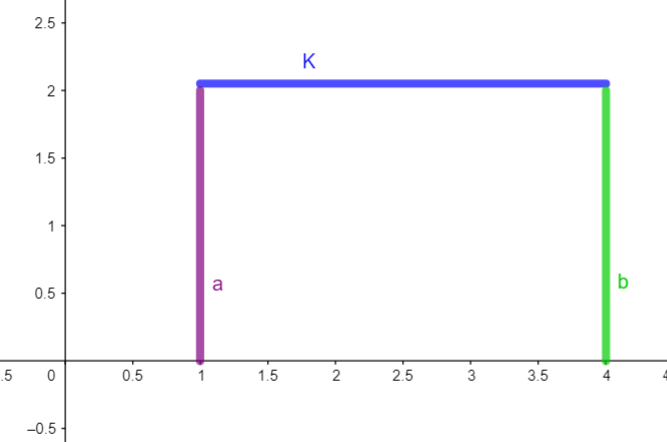
\includegraphics[scale=0.45]{images/uniform-distribution.png}
\end{figure}
\[f(x)= k,\ a\leq x \leq b\ \ \ \ \ \ \ \ \ Area=(b-a)k=1\ \ \ \ \ \ k=\frac{1}{b-a}\]
\[f(x) = \frac{1}{b-a} a \leq x \leq b\ \ \ \ \ \ \mu=E(x)=\frac{a+b}{2}\ \ \ \ \ \ Var(X)=\frac{(b-a)^2}{12}\]
\[Let\ a<b<c<d P(c\leq x \leq d)=\frac{d-c}{b-a};\ \ \ \ \ Area(c\leq x\leq d)=(d-c)k\]
\[P(c<x<d)=\frac{d-c}{b-a}=\frac{favourable\ length}{total\ length}\]


\subsection{Exponential Random Variable}
Exponential random variable function f(x) can be understood from the given figure.
\begin{figure}[h!]
    \centering
    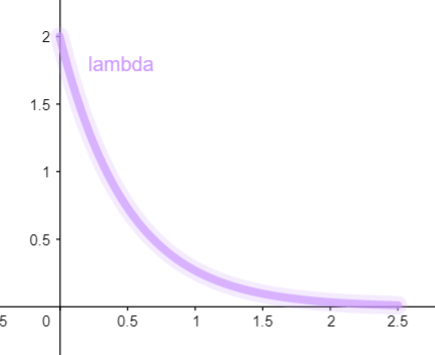
\includegraphics[scale=0.7]{images/exponential-random-variable.png}
\end{figure}
\[f(x)=\lambda e^{-\lambda x},\ x \geq 0\ \ \ \ \ \ \ E(x)=\frac{1}{\lambda};\ \ \ \ \ Var(x)=\frac{1}{\lambda^2}\]
For all Values of \(P(X\geq a)=e^{-\lambda a}\)


\subsection{Gauss or Normal Random Variable}
A Gauss Random Variable Function f(x) can be visualized as below.
\begin{figure}[h!]
    \centering
    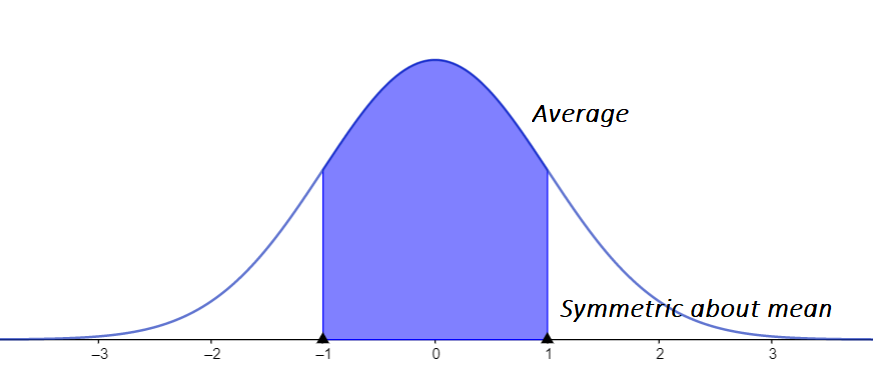
\includegraphics[scale=0.5]{images/normal-random-variable.png}
\end{figure}
\[f(x)=\frac{1}{\sigma \sqrt{2\pi}}e^{\frac{-(X-\mu)^2}{2\sigma^2}},\forall\ x\]


\subsection{Standard Normal Random Variable}
A normal random variable ``z'' is standard normal random variable if \(\mu=0,\ \sigma^2=1.\)
\[Let\ \emptyset(z)=P(Z\leq z)=\int_{-\infty}^z\frac{1}{\sqrt{2\pi}}e^{-{z^2/2}}\ dx\]
\[f(z)=\frac{1}{\sqrt{2\pi}}e^{-{z^2/2}}\ \ \ \ \ \ \ Y=ax+b\ \ \ \ E(Y)=aE(X)+b\ \ \ \ \ Var(X)=a^2Var(z)\]\vspace{0.2cm}\\

\begin{figure}[h!]
    \centering
    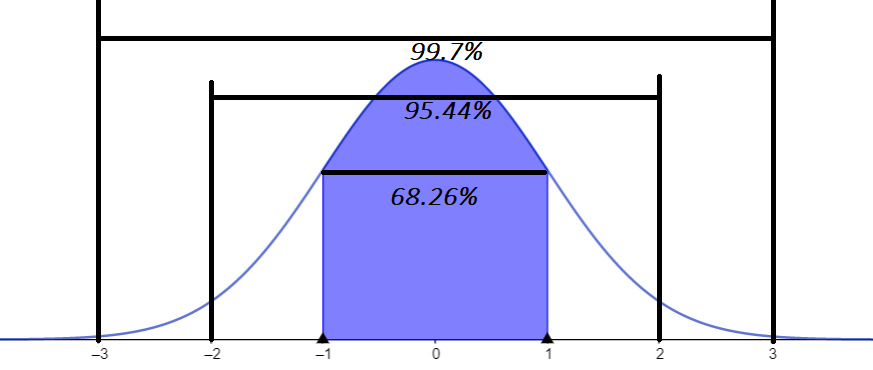
\includegraphics[scale=0.75]{images/standard-random-variable.png}
\end{figure}
\textbf{Key Points}
\begin{enumerate}
    \item The Normal distribution is symmetric about the mean.
    \item \(Area(X\leq\mu)=P(X\geq\mu)= \frac{1}{2}\)
    \item \(\int_{-\infty}^{\mu}f(x)\ dx=\int_{\mu}^{\infty}f(x)\ dx = \frac{1}{2}\)
    \item \(P(\mu-\sigma\leq X\leq \mu+\sigma)=68.26\%\)
    \item \(P(\mu-2\sigma\leq X\leq \mu+2\sigma)=95.44\%\)
    \item \(P(\mu-3\sigma\leq X\leq \mu+3\sigma)=99.7\%\)
\end{enumerate}

% Section 5
\chapter*{Numerical Methods}
\section{Numerical Methods}

\subsection{Linear Equations}
Consider the linear equations \(a_{11}x + a_{12}y + a_{13}z = b1; a_{21}x + a_{22}y + a_{23}z = b2; a_{31}x + a_{32}y + a_{33}z = b3;\)\\
A = 
$\begin{bmatrix}
a_{11} & a_{12} & a_{13}\\
a_{21} & a_{22} & a_{23}\\
a_{31} & a_{32} & a_{33}
\end{bmatrix}$\\
Diagnolly Dominant Matrix is defined as \[|a_{11}|\geq|a_{12}|+|a_{13}|\ \ \ \ \ |a_{22}|\geq|a_{21}|+|a_{23}|\ \ \ \ \ |a_{33}|\geq|a_{31}|+|a_{32}| \]
If the given matrix or equations are not in diagnol form then try re-arranging to obtain diagnolly dominant matrix.

\subsection*{Jacobi's Method}
Let initial guess be \(x_o, y_o, z_o\)
\[X_1=\frac{b_1-a_{12}y_o-a_{13}z_o}{a_{11}}\ \ \ Y_1=\frac{b_2-a_{21}x_o-a_{23}z_o}{a_{22}}\ \ \ Z_1=\frac{b_3-a_{31}x_o-a_{32}y_o}{a_{33}}\]

\subsection*{Gauss Seidel Method}
This method is twice faster than Jacobi's method because simultaneous substitutions. Let initial guess be \(x_o, y_o, z_o\)
\[X_1=\frac{b_1-a_{12}y_o-a_{13}z_o}{a_{11}}\ \ \ Y_1=\frac{b_2-a_{21}x_1-a_{23}z_o}{a_{22}}\ \ \ Z_1=\frac{b_3-a_{31}x_1-a_{32}y_1}{a_{33}}\]


\subsection{Non-Linear Equations}
If f(x)=0 is a transcedental equation, then y=f(x) is its corresponding curve.\\
If \(x = \alpha\) is the exact root of equation f(x)=0, then \(x=\alpha\) is the intersection of curve y=f(x) with x-axis.\\
If \(\alpha\) is the only root of the equation f(x)=0, between a and b then f(a) and f(b) must be of opposite sign else same sign.


\subsection*{Bisection/Bolzona Method}
In this method two initial approximation and has rate of convergence is One [linear].
\[C=\frac{a+b}{2}\]
After obtaining C value, then substitute C in f(x) to  get the next root and repeat it.
No of Iterations required to get the appropriate value is given by the formula
\[\frac{b-a}{2^n}\]

\subsection*{Regula Falsi Method}
This method is also known as method of false position. This method requires two initial approximation and the rate of convergence is One [Linear].
\[C= \frac{af(b)-bf(a)}{f(b)-f(a)}\]

\subsection*{Secant Method}
\[C = \frac{af(b)-bf(a)}{f(b)-f(a)}\ \ \ \ \ \ \ \ f(a) \& f(b) \text{ can have same sign}\]
\textbf{Difference between Secant and Regula Falsi Method}\\
After 1st Iteration the highest value of f(a) is eliminated in secant while the sign of f(a) is considered for elimination in regula falsi method.

\subsection*{Iterative Method}
In this method, Initial approximation is assumed (real value) and newton raphson's method is applied.

\subsection*{Newton-Raphson's Method}
This method is also known as method of tangents. This method requires one initial approximation and rate of convergence is two [Quadratic]. \(f'(x_n)-slope\ of\ tangent\)
\[x_{n+1}=x_n-\frac{f(x_n)}{f'(x_n)}\]

\textbf{Condition of Convergence of Newton-Raphson's Method}
\[\left|\frac{f(x_o).f''(x_0)}{[f'(x_o)]^2} \right| < 1\]

\subsection{Numerical Integration}
\subsection*{Trapezoidal Rule}
This method is also known as Composite or Complex Trapezoidal Rule.\\
\[\int_a^bf(x)\ dx=\frac{h}{2}[(y_0+y_n)+2(y_1+y_2+y_3+\ldots\ldots.+y_{n-1})]\]
\textbf{Simple Trapezoidal Rule} \[\int_a^bf(x)\ dx=\frac{h}{2}[(y_o+y_n)]\]

\subsection*{Simpson's Rule}
Order of Error = \(h^4\) and Accuracy \(O(h^4)\)\\
\textbf{1/3rd Rule}: if N is even (14/2)
\[\int_a^bf(x)\ dx=\frac{h}{3}[1(y_o+y_n)+4(y_1+y_3+y_5+\ldots\ldots.+y_{n-1})+2(y_2+y_4+\ldots\ldots.y_{n-2})]\]
\textbf{3/8th Rule}: if N is odd (13/2)
\[\int_a^bf(x)\ dx=\frac{3h}{8}[1(y_o+y_n)+3(y_1+y_2+y_4+\ldots\ldots.+y_{n-1})+2(y_3+y_6+\ldots\ldots.y_{n-3})]\]
For Both Trapezoidal Rule and Simpsons Rule, \(h=\frac{b-a}{n}\)
\begin{table}[h!]
\centering
\setlength{\tabcolsep}{1em}
\tabulinesep=2.5mm
\begin{tabu}{|c|c|}
\hline
\textbf{\begin{tabu}[c]{@{}c@{}}Order of \\ fitting Polynomial\end{tabu}}       & \textbf{Rule}        \\ \hline
1 (Linear for single Variable and hyperbolic for two variables)                 & Trapezoidal Rule     \\ \hline
2 (Parabolic)                                                                   & 1/3rd Simpson's Rule \\ \hline
3                                                                               & 3/8th Simpson's Rule \\ \hline
\end{tabu}
\end{table}

\subsection{Numerical Solutions of Oridinary Differential Equation}
\subsection*{Single Step Method}
\textbf{Taylor Series} - Consider a differential equation \(\frac{dy}{dx}=f(x,y)\) with initial condition \(y(x_o)=y_0,\ \ \ \ h=x-x_o\)
\[y_{n+1}=y_n+hy'_n + \frac{h^2}{2!}y''_n+ \frac{h^3}{3!}y'''_n+\ldots\ldots.\]
\textbf{Picard's Method of successive Approximation} - \(\frac{dy}{dx}=f(x,y)\ \ \ \ \ \ y_n = y_o+\int_{x_0}^xf(x,y_{n-1})\ dx\)

\subsection*{Multi step Method}
\textbf{Euler's Method} - For the differential Equation \(\frac{dy}{dx}=f(x,y)\) with initial conditions \(y(x_o)=y_o\), the euler's Iteration formula is
\[y_n = y_{n-1}+ hf(x_{n-1}, y_{n-1}),\ \ \ \ \ \ n=1,2,3\ldots\ldots. \]
\textbf{Modified Euler's Method}
\[y_n = y_{r-1}+\frac{h}{2}[f(x_{r-1}, y_{r-1})+f(x_r, y_r^{n-1})]\]
Iterations are repeated unless two successive approximation are appropriately equal.\vspace{0.2cm}\\
\textbf{Runge Kutta's Method}
\begin{table}[h!]
\centering
\setlength{\tabcolsep}{2em}
\tabulinesep=2.5mm
\begin{tabu}{|c|c|c|}
\hline
\textbf{Order} & \textbf{Equation}                      & \textbf{}                                                                                                                                                                                  \\ \hline
\textbf{1}     & \(y_0+hy_0'\)                          &                                                                                                                                                                                            \\ \hline
\textbf{2}     & \(y_0+\frac{1}{2}(k_1+k_2)\)           & \begin{tabu}[c]{@{}c@{}}\(k_1=hf(x_0, y_0)\)\\ \(k_2=hf(x_0+h,y_0+h)\)\end{tabu}                                                                                                     \\ \hline
\textbf{3}     & \(y_0+\frac{1}{6}(k_1+4k_2+k_3)\)      & \begin{tabu}[c]{@{}c@{}}\(k_1=hf(x_0, y_0)\)\\ \(k_2=hf(x_0+\frac{h}{2},y_0+\frac{k_1}{2})\)\\ \(k_3=hf(x_0+h,y_0+k_2)\)\end{tabu}                                                   \\ \hline
\textbf{4}     & \(y_0+\frac{1}{6}(k_1+2k_2+2k_3+k_4)\) & \begin{tabu}[c]{@{}c@{}}\(k_1=hf(x_0, y_0)\)\\ \(k_2=hf(x_0+\frac{h}{2},y_0+\frac{k_1}{2})\)\\  \(k_3=hf(x_0+\frac{h}{2},y_0+\frac{k_2}{2})\)\\  \(k_4=hf(x_0+h,y_0+k_3)\)\end{tabu} \\ \hline
\end{tabu}
\end{table}
